\documentclass[openright,twoside,10pt]{memoir}
%
% Packages
%
%\usepackage[utf8]{inputenc}
\usepackage[T1]{fontenc}
\usepackage[danish]{babel}
\linespread{1.05}
\usepackage{fontspec}

\setmainfont[Ligatures=TeX]{Garamond}
\setmonofont{Consolas}
% Eksempel
%\newfontfamily{\titlefont}{Antique-Olive Th}

%\newcommand{\heading}[1]{ \vspace{0.5cm} {\titlefont \Large #1}\\ }
%\newcommand{\bilagtitle}[1]{ {\titlefont \LARGE #1}\\ }

%---- 

\usepackage{tocloft}
\usepackage{courier}

\chapterstyle{hangnum}
\raggedbottom
\setlength{\beforechapskip}{0pt}
\setlength{\afterchapskip}{10pt} % vspace under chapters
\setlength{\belowcaptionskip}{-7pt} % vspace mellem caption og tekst
\setsecnumdepth{subsection}

\renewcommand*{\partnamefont}{\normalfont\Huge\bfseries}
\renewcommand*{\partnumfont}{\normalfont\Huge\bfseries}
\renewcommand*{\parttitlefont}{\normalfont\HUGE\bfseries}
\renewcommand*{\chaptitlefont}{\normalfont\HUGE\bfseries}
\setsecheadstyle{\normalfont\huge\bfseries}
\setsubsecheadstyle{\normalfont\Large\bfseries}
\setsubsubsecheadstyle{\normalfont\large\bfseries}

%% Fonts
%\usepackage[sc]{mathpazo}
%\usepackage{courier}
%\usepackage{inconsolata}
%\usepackage[scaled]{uarial}
%\renewcommand*\familydefault{\sfdefault}

% En pil...
\usepackage{textcomp}

\usepackage{multirow}
\usepackage{tabularx}
\usepackage{icomma}
\usepackage{amsmath,amsfonts,amssymb}
\usepackage{mathtools}
\usepackage{graphicx}
\usepackage{gensymb}
\usepackage[usenames,dvipsnames,table]{xcolor} % til farvning af celler i tabel
\usepackage{url}
%\usepackage[bottom]{footmisc} % keep footnotes at bottom UNCOMMENTED
%PGA errors
\usepackage{bbding}
\usepackage{pdfpages}
\usepackage{float} %kan bruge H placement modifier, bedre end "h!"
%\usepackage{wrapfig}
\usepackage{subfig}
%\usepackage{sagetex}
\usepackage[section]{placeins}
\usepackage{xspace}
\usepackage[chapter]{algorithm}
\usepackage{algpseudocode}
\usepackage{algorithmicx}

\parskip=5pt plus 2pt minus 1pt
\parindent=0pt
\frenchspacing % kommeretninger

% Fancy ting med enheder og datatabeller. Læs manualen til pakken
% Manual: http://www.ctan.org/tex-archive/macros/latex/contrib/siunitx/siunitx.pdf
\usepackage{siunitx}

%\usepackage{siunitx}
%\usetikzlibrary{shapes}
\usepackage{enumitem} %stackoverflow.com/questions/3275622/latex-remove-spaces-between-items-in-list
\usepackage{listings}
%\setcounter{secnumdepth}{3}
%\setcounter{tocdepth}{3}

\definecolor{shcomment}{rgb}{0.12, 0.38, 0.18 }
%adjusted, in Eclipse: {0.25, 0.42, 0.30 } = #3F6A4D
\definecolor{shkeyword}{rgb}{0.37, 0.08, 0.25}  % #5F1441
\definecolor{shstring}{rgb}{0.06, 0.10, 0.98} % #101AF9

\setfloatlocations{figure}{htb}

 \lstset{ % http://stackoverflow.com/questions/741985/latex-source-code-listing-like-in-professional-books
%         basicstyle=\footnotesize\ttfamily,% the size of the fonts
                                % that are used for the code
        basicstyle=\footnotesize\ttfamily,% the size of the fonts that are used for the code
         numbers=left,                     % where to put the line-numbers
         numberstyle=\tiny,                % the size of the fonts that are used for the line-numbers
         stepnumber=1,                     % line numbering steps
         numbersep=5pt,                    % how far the line-numbers are from the code
         tabsize=2,                        % sets default tabsize to 2 spaces
         breaklines=true,                  % sets automatic line breaking
         keywordstyle=\color{shkeyword},        % language function text color
    		frame=b,
 %        keywordstyle=[1]\textbf,    % Stil der Keywords
 %        keywordstyle=[2]\textbf,    %
 %        keywordstyle=[3]\textbf,    %
 %        keywordstyle=[4]\textbf,   \sqrt{\sqrt{}} %
         stringstyle=\color{shstring}, % string text color
%         stringstyle=\color{red},
        commentstyle=\color{shcomment},
         showspaces=false,           % show spaces adding particular underscores
         showtabs=false,             % show tabs within strings adding particular underscores   
         showstringspaces=false,     % underline spaces within strings
         xleftmargin=17pt,
         framexleftmargin=17pt,
         framexrightmargin=5pt,
         framexbottommargin=4pt,
         language=Ruby
 }
    %\DeclareCaptionFont{blue}{\color{blue}} 

%\captionsetup[lstlisting]{singlelinecheck=false, labelfont={blue}, textfont={blue}}
\DeclareCaptionFont{white}{\color{white}}
\DeclareCaptionFormat{listing}{\hrule\smallskip\parbox{\textwidth}{\hspace{15pt}#1#2#3}\smallskip\hrule}
\captionsetup[lstlisting]{format=listing,
  singlelinecheck=false, margin=0pt, font={bf,footnotesize}}



\usepackage{memhfixc}
%
% Fra AAU temp
%
\usepackage{calc}
\usepackage{lastpage}

\usepackage{hyperref}
%
% Layout
%
\newenvironment{indledning}{\sffamily}{\vskip 0.75cm}
\newenvironment{tail}{\vskip 0.75cm\itshape}{}
\newcommand{\spc}[1] {#1 \vskip 1cm}
\definecolor{aaublue}{HTML}{0492D2}

\let\oldmarginpar\marginpar
\renewcommand\marginpar[1]{\-\oldmarginpar[\raggedleft\footnotesize #1]%
{\raggedright\footnotesize\color{red} #1}}
% Margins
\setstocksize{11in}{8.5in}
\settrimmedsize{11in}{8.5in}{*}
\settrims{0in}{0in}
\settypeblocksize{9.0in}{6in}{*}
\setlrmargins{1.25in}{*}{*}
\setulmargins{1.0in}{*}{*}
\setheadfoot{14pt}{26pt}
\setheaderspaces{*}{13pt}{*}

% Fra settings.tex
\setlrmarginsandblock{3.5cm}{2.5cm}{*}
\setulmarginsandblock{2.5cm}{3.0cm}{*}

\checkandfixthelayout
%
% Tikz
%
%\tikzstyle{block}=[draw, rectangle, text width=2cm, minimum height=1cm, text badly centered, node distance=\afs]
%\tikzstyle{cloud}=[draw, ellipse, minimum width=2cm, fill=gray!40]
%\tikzstyle{valg} = [draw, diamond, inner sep=1pt, text badly centered, text width=4.5em]
%\tikzstyle{pil} = [draw, -latex]

\setlength{\unitlength}{2em} % for the picture environment

\usepackage[compact]{titlesec}
\titlespacing{\section}{0pt}{*0}{*0}
\titlespacing{\subsection}{0pt}{*0}{*0}
\titlespacing{\subsubsection}{0pt}{*0}{*0}

% Forhindrer horeunger..:

\widowpenalty=300
\clubpenalty=300

\setlength{\parskip}{3ex plus 2ex minus 2ex}

%extra colonner til titelbladet
\usepackage{multicol}

% procenttegn
\let\oldpercent=\%
\renewcommand{\%}{\ifmmode\ \oldpercent\else\oldpercent\fi}

%
% Check-in by Niels on November 07
%
% Alter some LaTeX defaults for better treatment of figures:
    % See p.105 of "TeX Unbound" for suggested values.
    % See pp. 199-200 of Lamport's "LaTeX" book for details.
    %   General parameters, for ALL pages:
    \renewcommand{\topfraction}{0.9}	% max fraction of floats at top
    \renewcommand{\bottomfraction}{0.8}	% max fraction of floats at bottom
    %   Parameters for TEXT pages (not float pages):
    \setcounter{topnumber}{2}
    \setcounter{bottomnumber}{2}
    \setcounter{totalnumber}{4}     % 2 may work better
    \setcounter{dbltopnumber}{2}    % for 2-column pages
    \renewcommand{\dbltopfraction}{0.9}	% fit big float above 2-col. text
    \renewcommand{\textfraction}{0.07}	% allow minimal text w. figs
    %   Parameters for FLOAT pages (not text pages):
    \renewcommand{\floatpagefraction}{0.7}	% require fuller float pages
	% N.B.: floatpagefraction MUST be less than topfraction !!
    \renewcommand{\dblfloatpagefraction}{0.7}	% require fuller float pages


% Degrees
%\newcommand{\degree}{\ensuremath{^\circ}}
\DeclareMathOperator*{\argmax}{arg\,max}


% References
\newcommand{\secref}[1]{afsnit \ref{#1}}
\newcommand{\chapref}[1]{kapitel \ref{#1}}
\newcommand{\figref}[1]{figur \ref{#1}}
\newcommand{\lstref}[1]{eksempel \ref{#1}}
\newcommand{\apref}[1]{bilag \ref{#1}}
\newcommand{\tableref}[1]{tabel \ref{#1}}
\newcommand{\itemref}[1]{element \ref{#1}}
\newcommand{\coderef}[1]{eksempel \ref{#1}} % deprecated, use \lstref
\newcommand{\pseudoref}[1]{algoritme \ref{#1}}

\newcommand{\fileref}[1]{\texttt{#1}}
\newcommand{\classref}[1]{\textcolor{classcolor}{\texttt{#1}}}
\newcommand{\methodref}[1]{\textcolor{methodcolor}{\texttt{#1}}}
\newcommand{\dbtableref}[1]{\texttt{#1}}
\newcommand{\classmethodref}[2]{\classref{#1}\texttt{.}\methodref{#2}}

\newcommand{\tablespacing}{\newline \qquad \newline}

\floatname{algorithm}{Algoritme}
\renewcommand\lstlistingname{Eksempel}
\renewcommand\lstlistlistingname{Eksempler}

% Other
\newcommand{\capt}[1]{\caption{\emph{#1}}} % Emphesize caption
\newcommand{\arrows}[2]{#1$\Leftrightarrow$#2} % Pil mellem to inputs
\newcommand{\op}[1]{$\Uparrow$ #1} % Pil op
\newcommand{\ned}[1]{$\Downarrow$ #1} % Pil ned

%\titleformat{\subparagraph}
%    {\normalfont\normalsize\bfseries}{\thesubparagraph}{1em}{}
%\titlespacing*{\subparagraph}{\parindent}{3.25ex plus 1ex minus .2ex}{.75ex plus .1ex}

\newcommand{\skippar}{}

\newcommand{\fx}{f.eks. }
\newcommand{\Fx}{F.eks. }

\newcommand{\informantet}{informant1}
\newcommand{\Informantet}{Informant1}
\newcommand{\informantto}{informant2}
\newcommand{\Informantto}{Informant2}
\newcommand{\ooadbog}{Objektorienteret Analyse \& Design}

% Til hændelsestabellen
\newcommand{\once}{\texttt{+}}
%\newcommand{\iter}{\textasteriskcentered}
\newcommand{\iter}{$\circlearrowleft$}

\newcommand{\Foodl}{{\color{OliveGreen}\sffamily foodl}}

\newcommand{\todo}[1]{\colorbox{yellow}{\color{red}\textbf{TODO} \hspace{1ex} #1}}
\newcommand{\tjek}[1]{\colorbox{yellow}{\color{red}\textbf{LÆS MIG:} \guillemotright #1 \guillemotleft}}


\newlength{\tablewidth}
\setlength{\tablewidth}{\textwidth}
\addtolength{\tablewidth}{-12pt}

\newcommand{\tabelmedoverskrift}[3]{
\subsubsection{#1}
\label{sec:#2}
#3}

\newcommand{\aktortabel}[4]{\tabelmedoverskrift{#1}{#2}{\textbf{Formål:} #3
 
\textbf{Karakteristik:} #4}}

\newcommand{\aktortabelEx}[5]{\aktortabel{#1}{#2}{#3}{#4 

\textbf{Eksempler:} #5}}


\newcommand{\pdffig}[4][0.9]{\begin{figure}[H]
  \centering
  \sffamily
  \scalebox{#1}{
    \input{billeder/#2.pdf_tex}
  }
  \capt{#3}
  \label{#4}
\end{figure}}

\newcommand{\brugtabel}[6]{\tabelmedoverskrift{#1}{#2}{\textbf{Brugsmønster:} #3

\textbf{Objekter:} #4

\textbf{Funktioner:} #5}
\pdffig[0.9]{brugsmoenstre/#2}{#6}{fig:bm-#2}
}

% Table stuff!!!
\newcommand{\ourtable}[7]{
\begin{table}[H]
  \centering
    \begin{tabularx}{\textwidth}{ r | >{\centering\arraybackslash}X>{\centering\arraybackslash}X>{\centering\arraybackslash}X>{\centering\arraybackslash}X>{\centering\arraybackslash}X>{\centering\arraybackslash}X>{\centering\arraybackslash}X>{\centering\arraybackslash}X>{\centering\arraybackslash}X>{\centering\arraybackslash}X>{\centering\arraybackslash}X>{\centering\arraybackslash}X>{\centering\arraybackslash}X>{\centering\arraybackslash}X>{\centering\arraybackslash}X>{\centering\arraybackslash}X>{\centering\arraybackslash}X>{\centering\arraybackslash}X>{\centering\arraybackslash}X>{\centering\arraybackslash}X>{\centering\arraybackslash}X>{\centering\arraybackslash}X>{\centering\arraybackslash}X>{\centering\arraybackslash}X>{\centering\arraybackslash}X>{\centering\arraybackslash}X>{\centering\arraybackslash}X>{\centering\arraybackslash}X>{\centering\arraybackslash}X>{\centering\arraybackslash}X>{\centering\arraybackslash}X } %Errr, doesn't seem to give any errors, but fix it if possible
  \hline
  & \multicolumn{#2}{c}{\textbf{#4}} \\
   \textbf{#5}    & #6 \\ \hline
	#7
	\hline
    \end{tabularx}
    \capt{#3}
    \label{table:#1}
\end{table}
}

\newcommand{\ourrow}[2]{ #1 & #2 \\ }


\begin{document}

\setcounter{page}{-100}
\pagenumbering{roman}
\frontmatter
\selectlanguage{danish}
\pagestyle{empty}
\subsection{Forside}
\label{subsec:brug-forside}

Når man taster sig ind på hjemmesiden \url{http://www.foodl.dk}, bliver man mødt af en velkomsthilsen, der meget kort beskriver hjemmesidens formål og brug, som kan ses på \figref{fig:overblik-forside}. Denne hilsen kan brugeren vælge at lukke ned. En cookie bliver gemt i browseren, så velkomsthilsnen ikke bliver vist igen, medmindre browserhistorikken bliver ryddet.

\begin{figure}[H]
	\centering
	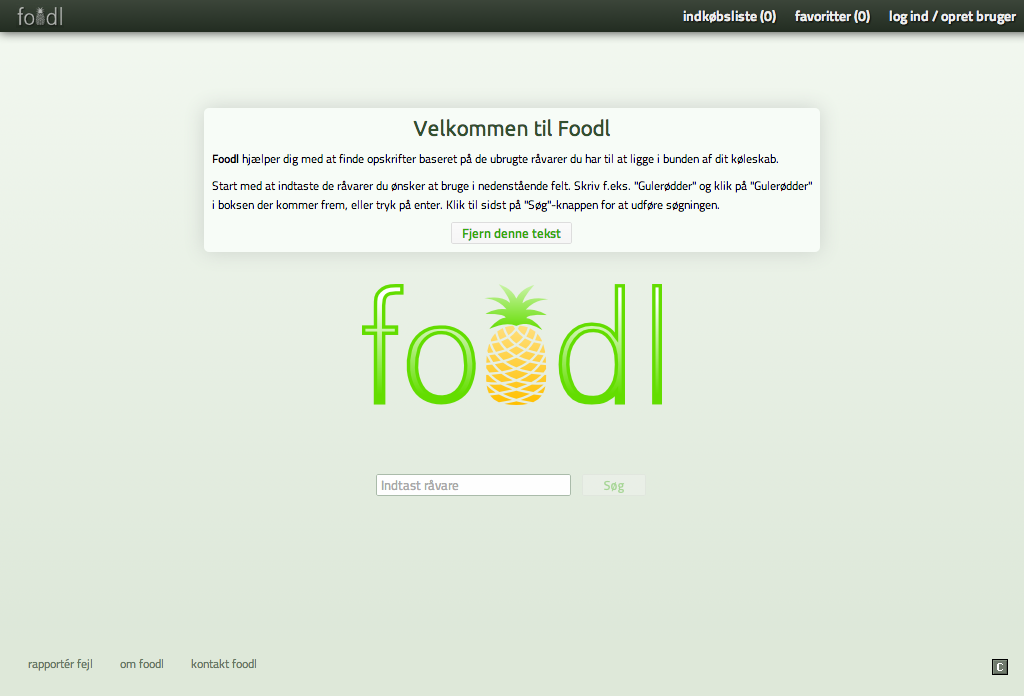
\includegraphics[scale=1]{billeder/foodl/thumbnails/forside.png}
	\capt{Denne figur har til formål at give et overblik over systemets forside.}
	\label{fig:overblik-forside}
\end{figure}

Navnet \Foodl{} er også en del af webapplikationens logo. For at gøre det klarere for en ny bruger, hvad siden handler om, erstattede vi et O i navnet med en stor ananas, fordi det er noget, der kan spises, og sidens formål er at give folk mulighed for at genbruge deres madrester. 

På toppen af alle undersider af \Foodl{} er det muligt at tilgå sidehovedet. Her er der mulighed for at navigere tilbage til forsiden ved at klikke på den mindre version af det store logo. Derudover kan man tilgå både en indkøbsliste, der er nærmere beskrevet i \secref{subsec:brug-indkoebsliste}, og en liste af favorit-opskrifter, som brugeren selv vælger fra hjemmesiden. Favoritlisten bliver beskrevet nærmere i \secref{subsec:brug-favoritliste}. Både indkøbslisten og favoritter har et tal i parentes, der fortæller brugeren, hvor mange varer, der er i den nuværende indkøbsliste, eller hvor mange opskrifter, der er gemt under favoritter. Dette kan ses påtoppen af \figref{fig:overblik-forside}. På sidehovedet kan man også logge ind i systemet eller oprette en bruger, hvilket er forklaret nærmere i \secref{subsec:brug-brugeroprettelse}.

Efter brugeren føler sig tryg ved hjemmesiden og evt. har lukket velkomsthilsnen ned, så er det tid til at indtaste alle de råvarer, der ønskes brugt til madlavningen. Figur \ref{fig:foodl-soegefelt} viser, hvordan en sådan søgning foregår. Der bliver løbende indtastet bogstaver, og systemet undersøger for dele af tekststrenge, der matcher det, som bliver indtastet. Ud fra disse match gives der forslag til hvilke råvarer, man kan vælge. Man kan ikke indtaste, hvad som helst som et søgekriterie i systemet. Der er en lang række råvarer at vælge imellem. Hvis der \fx bliver indtastet kød i søgefeltet, så kommer der en liste af matchende råvarer som forslag, som man kan se på \figref{fig:foodl-soegefelt}. Der er ingen begræsning for, hvor mange råvarer, der kan indtastes som søgekriterier.

\begin{figure}[H]
	\centering
	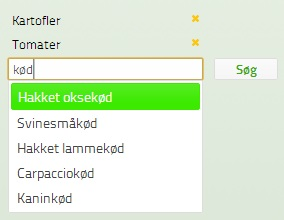
\includegraphics[scale=0.7]{billeder/foodl/soegefelt.jpg}
	\capt{Denne figur viser systemets søgefelt.}
	\label{fig:foodl-soegefelt}
\end{figure}


For at fuldføre en søgning skal man blot trykke på ``Søg'', der er til højre for søgefeltet. Når brugeren trykker ``Søg'', så arbejder systemet på at finde alle de opskrifter, der minimum har én ingrediens, der matcher en af de indtastede råvarer. Det er efter sådan en søgning, at brugeren finder ud af, hvad der er muligt at lave ud fra de råvarer, der er til rådighed (resultatet er afgrænset til den database, man har over opskrifter).
%\clearpage
\begin{nopagebreak}
\LARGE{\textbf{Det Teknisk-Naturvidenskabelige Fakultet}}\vspace{-0.9cm}

\large{\textbf{Datalogi}}
\hspace{10.5cm}
\includegraphics[height=0.75cm]{billeder/aau_logo.pdf}


\hrule

\newcommand{\titleitem}[2]{\textbf{#1:}

\hspace*{0.5cm}
\begin{minipage}{0.9\columnwidth}#2\end{minipage}
\vspace{0.25cm}}
\begin{multicols}{2}

  \titleitem{Titel}{
\includegraphics[width=3.65cm]{billeder/logo.png}\\Anvendelse af Madrester}

\titleitem{Tema}{Udvikling af applikationer – fra brugere til data, algoritmer og test – og tilbage igen}

\titleitem{Projektperiode}{P3, 3. september - 20. december 2012}

\titleitem{Projektgruppe}{d303e12 (\url{d303e12@cs.aau.dk})}

\titleitem{Deltagere}{
    Sebastian Wahl\\
    Simon Buus Jensen\\
    Elias Khazen Obeid\\
    Niels Sonnich Poulsen\\
    Kent Munthe Caspersen\\
    Martin Bjeldbak Madsen
}

\titleitem{Vejleder}{Lise T. Heeager}

% Tilføj senere
% \titleitem{Sidetal}{\pageref{sidsteSideUdenBilag}} 
% \titleitem{Sidetal m/ bilag} {\pgeref{sidsteSideMedBilag}}
\titleitem{Afsluttet}{20. december 2012}

\vfill
\columnbreak

\titleitem{Synopsis}{ Denne rapport gør rede for udviklingsprocessen bag produktionen af systemet \Foodl{}, der er en webapplikation. 
Undersøgelser viser, at personer, der bor i parcelhuse, smider i gennemsnit 42 kg mad ud om året.
\Foodl{} har til formål at gøre det lettere for de madansvarlige i de danske husstande at genbruge madrester fra bl.a. gårsdagens aftensmad for at mindske spildet af mad.

Igennem en iterativ udviklingsmetode har vi analyseret, designet, implementeret og testet systemet.
Vi benyttede en objektorienteret metode, der er blevet præsenteret i bogen Objektorienteret Analyse \& Design \cite{ooad}.
Til udvikling af systemet havde vi et tæt samarbejde med to informanter, der hjalp os med at fortolke og revidere problemstillingen. Informanterne var en stor del af analysen, designet og kvalitetssikringen af systemet.

I konklusionen har vi konkluderet, at \Foodl{} gør det lettere for de madansvarlige at få inspiration til at genbruge madrester.
Vi har, i perspektiveringen, reflekteret over, hvad der kan gøre systemet endnu bedre. }

\end{multicols}
\centering
\textit{Rapportens indhold er frit tilgængeligt, men offentliggørelse (med kildeangivelse) må kun ske efter aftale med
forfatterne.}

\end{nopagebreak}

\cleardoublepage
\pagestyle{ruled}
\section{Forord}


\tableofcontents*
%--Clear page
%\newpage
%\thispagestyle{empty}
%\hspace{1cm}
%\newpage
%--
\cleardoublepage

\pagenumbering{arabic}
\mainmatter
\part{Udviklingsrapport}
\begin{frame}
\frametitle{Problemstilling}

	\textbf{Hvorfor madspild?}
	\begin{itemize}
		\item Interessant og relevant
	\end{itemize}
	
	\textbf{Industrien i vestlige lande:}
	\begin{itemize}		
		\item 30 \% 
		\begin{itemize}
			\item Forkert størrelse
			\item Forkert udseende
			\item Spiselig mad
		\end{itemize}
	\end{itemize}	
	\textbf{Privatpersoner:}	
	\begin{itemize}
		\item 42 kg/år
		\item 40 \% eneboende i Danmark
		\item Portionsstørrelse
		\item Fryse eller genbruge madrester
	\end{itemize}
	
%	\begin{quote}
%	``I am a single person and I do waste a lot simply because
%	of packaging. I don't know what \% of people are single
%	but I either haev to freeze stuff if I can or eat the
%	same dish 2-3 days.'' - Dee Simmons
%	\end{quote}

\end{frame}
\chapter{Analyse af problemområdet}
\label{chap:analyseafpo}

Analysen tager udgangspunkt i en metode fra bogen Objektorienteret Analyse \& Design (OOAD)\cite[s. ~43]{ooad}. Problemområdet er den del af omgivelserne, som skal administreres, styres og overvåges af vores system. I vores tilfælde er problemområdet: madresterne og madlavningen i de danske hustande. Formålet med analysen er at skabe et overblik over, hvilke klasser og hændelser systemet skal have, for at kunne udføre de funktioner, vi ønsker, og for at systemet bliver så brugbart som muligt for dets fremtidige brugere. 

Vi har valgt at dele analysen op i følgende fire aktiviteter: identificering og udvælgelse af klasser og identificering og udvælgelse af hændelser, som beskrives i \secref{sec:klasser}. Strukturering af klasser og hændelser (struktureres vha. et klassediagram), som beskrives i \secref{sec:struktur}, og analyse og beskrivelse af adfærdsmønstre for klasserne, som beskrives i \secref{sec:adfaerd} vha. tilstandsdiagrammer. Resultatet af de fire aktiviteter er en hændelsestabel, som ses i \tableref{table:haendelsestabel}, der er præsenteret i slutningen af \secref{sec:klasser} for at give et overblik over, hvad der kommer i de efterfølgende afsnit i dette kapitel.

% Problemområde
\section{Klasser}
\label{sec:klasser}

En klasse er en beskrivelse af en samling af objekter med samme struktur, adfærdsmønster og attributter \cite[s. ~51]{ooad}. To klasser kan have en association mellem dem, men det er ikke altid helt klart, hvad denne association skal betyde. Vi har løst dette problem ved at navngive nogle af associationerne mellem klasser. Ser vi på \figref{fig:klassediagram} i \secref{sec:struktur}, så ser vi eksempler på navngivne associationer. Her er en ``Vare'' associeret med en ``Person'', og associationen er navngivet ``Indkøbsliste''. 

Overblikket over hvilke klasser systemet skal have, kan skabes ved først at finde så mange klasserkandidater som muligt, og dernæst at afgrænse disse, så kun de mest relevante klasser er tilbage. I vores tilfælde anvendte vi en kombination af rigebilleder, som kan ses i \figref{fig:rigbillede1} og \figref{fig:rigbillede2}, samt systemdefinitionen som hjælpemidler til at finde frem til de klasser, som vi vil modellere i problemområdet.

Grundet den evolutionære arbejdsmetode, som vi har arbejdet ud fra, er klasser undervejs i forløbet blevet tilføjet og fjernet. De klasser som er blevet fravalgt, kan ses i \apref{ap:fravalgteklasser}. Herunder ses de valgte klasser, samt beskrivelser og begrundelser for, hvorfor de er med i vores problemområde.

\begin{description}
\item[Person] \hfill \\
En person er en, der er ansvarlig eller hjælper til med madlavningen i husstanden. En person kan være i besiddelse af en indkøbsliste, der bruges til at håndtere fremtidige indkøb af varer. Derudover kan en person have bogmærket nogle opskrifter, som vedkommende synes godt om.

\item[Opskrift] \hfill \\
En opskrift er den centrale klasse i problemområdet. En opskrift kan findes i en opskriftsamling, i en kogebog eller på nettet. Opskrifter indeholder en ingrediensliste. En opskrift kan være ikke-bogmærket eller bogmærket, hvis en person ønsker, at opskriften skal være let tilgængelig eller ej.

\item[Råvaretype] \hfill \\
En råvaretype findes i køleskabene, på madhylderne i husstanden og i supermarkederne. Råvaretype adskiller sig fra klassen ingrediens, ved at en råvaretype ikke har nogen enhed eller mængde. Et eksempel på råvaretyper kunne være ``gulerødder'', ``mælk'', ``hakket oksekød'' osv. 

\item[Ingrediens] \hfill \\ 
En ingrediens tilhører en råvaretype, og består af en mængde og en enhed. En ingrediens kan befinde sig på en ingrediensliste på en opskrift. Klassen ingrediens skiller sig ud fra råvaretype, netop fordi den udover at være en råvaretype, også har en mængde og en enhed. Eksempler på ingredienser er: ``3 styk gulerødder'', ``4 liter mælk'', ``500 gram hakket oksekød'' osv.

\item[Vare] \hfill \\
En vare er en vare som man kender det fra supermarkeder. En vare, i modsætning til ingredienser, tilhører ikke en råvaretype. En vare kan \fx være toiletpapir, vaskepulver eller blyanter. En vare kan befinde sig på en persons indkøbsliste.

\item[Fejl] \hfill \\
Fejl opstår som \fx en mængdefejl i en opskrift eller en manglende instruktion i fremgangsmåden. Fejl er uventede, og det er svært at sige, hvor de opstår og i hvilket omfang.

\end{description}

Ud fra de valgte klasser, skal vi have formuleret nogle hændelser, som beskriver klassernes adfærd. For klassen ``opskrift'', kan en hændelse \fx være ``opskrift fundet''. En hændelse er en bestemt adfærd for en klasse, som beskrives med udsagnsord. En hændelse kan involvere en til flere klasser. Som i eksemplet før, så involverer hændelsen ``opskrift fundet'', både ``opskrift'' men også ``ingrediens'', da vi vurderer, at man skal finde en opskrift før man kan arbejde med ingredienser, fordi en opskrift består af ingredienser. Ligesom med klasser, så har vi gennem forløbet, pga. den evolutionære arbejdsmetode, tilføjet og fjernet hændelser, igen og igen. De hændelser, som er blevet fravalgt, kan ses i \apref{ap:fravalgteklasseroghaendelser}.

I \tableref{table:haendelsestabel} ses de valgte hændelser, og hvilke klasser, disse hændelser, har en indflydelse på. Hver hændelse forårsager et tilstandsskift, og disse tilstande kan ses i tilstandsdiagrammerne i \secref{sec:adfaerd}. Hændelsestabellen er resultatet af analysen af problemområdet, men vi præsenterer den allerede nu, da den giver et godt overblik over de hændelser og klasser, vi er endt op med. 

I hændelsestabellen benytter vi \iter-symbolet til at illustrere, at den tilhørende hændelse kan forekomme flere gange i den pågældende klasse. Det betyder, at denne hændelse kan ses som en iteration i tilstandsdiagrammerne i \secref{sec:adfaerd}. Derudover benytter vi \once-symbolet til at illustrere, at den tilhørende hændelse blot kan forekomme en gang i klassen. Det betyder, at hændelsen kan ses som en selektion eller en sekvens i tilstandsdiagrammerne.

\ourtable{haendelsestabel}{5}{Hændelsestabel for klasserne person, opskrift, ingrediens, råvaretype, vare og fejl}
                                                             {Klasser}
       {Hændelser             	}{ Opskrift & Person & Vare  & Ingrediens & Råvaretype & Fejl  }{
\ourrow{Opskrift smidt ud     	}{ \once    &        &       & \once      &            &       }
\ourrow{Opskrift fundet         }{ \once    &        &       & \once      &            &       }
\ourrow{Bogmærke sat ind      	}{ \iter    & \iter  &       &            &            &       }
\ourrow{Bogmærke fjernet      	}{ \iter    & \iter  &       &            &            &       }
\ourrow{Skrevet på indkøbsliste	}{ \iter    & \iter  & \once & \iter      &            &       }
\ourrow{Fjernet fra indkøbsliste}{          & \iter  & \once & \iter      &            &       }
\ourrow{Råvare opbrugt        	}{          &        &       &            & \iter      &       }
\ourrow{Råvare købt           	}{          &        &       &            & \iter      &       }
\ourrow{Fejl rapport\'{e}ret    }{ \iter    & \iter  &       &            &            & \once }
\ourrow{Tilbagemelding modtaget }{          & \once  &       &            &            & \once }
\ourrow{Fejl set bort fra       }{          &        &       &            &            & \once }
}


Problemområdet består af madrester og madlavning i husstanden, derfor er det vigtigt, at problemområdet bliver repræsenteret ordentligt, i form af klasser. Madlavning, skal ikke forståes, som at vi ønsker at overvåge, om der bliver lavet mad i husstanden, da det vi ønsker blot er at udvikle et system, der giver mulighed for at genbruge madrester, og give inspiration til madlavningen.
 
\section{Struktur}
\label{sec:struktur}

Der kan opbygges en struktur imellem de forskellige klasser. Dette kan ses i \figref{fig:klassediagram}. 

\begin{figure}
  \centering
  \input{billeder/klasseDiagram.pdf_tex}
  \capt{Klassediagram for problemområdet.}
  \label{fig:klassediagram}
\end{figure}


Klassediagrammet ovenover er bygget op af aggregeringer og associationer imellem klasserne i diagrammet. Hierakimønsteret benyttes idet at en indkøbsliste består af 0 til mange ingredienser, som hvor især består af en råvare. Hver enkelt klasses forbindelse forklares her nærmere:

\begin{description}
  \item[Bogmærke] \hfill \\
    Et bogmærke er associeret med netop én opskrift. Multipliciteten er valgt på baggrund af at et bogmærke kan sættes på én og kun én side i en kogebog.

  \item[Opskrift] \hfill \\
    En opskrift kan være associeret med 0 eller 1 bogmærke. Man kan argumentere for, at der godt kan placeres flere bogmærker på samme opskrift, men vi ønsker kun at overvåge hvorvidt en opskrift er bogmærket eller ej, og det er derfor kun nødvendigt at skelne mellem 0 og 1 bogmærker. En opskrift består af 1 til flere ingredienser. Hvis opskriften ikke bestod af ingredienser, ville det ikke være en opskrift.

\item[Indkøbsliste] \hfill \\
  En indkøbslisten består af 0 til flere ingredienser. 0 er muligt, da indkøbslisten er tom inden man tilføjer ingredienser til den. Det kan også være at man starter med bare at skrive ``Jeg handler ind kl. 17, skriv hvad jeg skal købe - Farmand'', og lader resten af familien udfylde sedlen.

\item[Ingrediens] \hfill \\
  En ingrediens består af netop én råvare og aggregeres altid af kun én opskrift. Selvom flere opskrifter indeholder oksekød, kan mængden være forskellig. Samtidig er det logisk, at hvis to opskrifter begge indeholder en ingrediens \textit{400 g oksekød}, så kan den ene opskrift ændres til \textit{500 g oksekød}, uden at den anden opskrift skal ændres.

\item[Råvare] \hfill \\
  En råvare er en dekomponering af en ingrediens. En råvare er blot en ingrediens uden nogen form for information om mængde eller enhed. En ingrediens kunne for eksempel være \textit{400 g oksekød}, som består af råvaren \textit{oksekød}.
\end{description}

            
\section{Adfærd}
\label{sec:adfaerd}

Den sidste aktivitet i analyse af problemområdet, består i at analysere og beskrive adfærdsmønstre for klassers objekter. Formålet med dette, er at få en bred for forståelse af, hvordan objekter kan opføre sig, hvilket vi vil bruge senere, når vi skal beskrive de funktioner \Foodl{} skal have. Dermed opnåes der også en mere glidende overgang over mod analyse af anvendelsesområdet \chapref{chap:analyseafao}. Desuden har vi anvendt adfærdmønstrene til at få overblik over, om de hændelser vi har valgt, er fyldestgørende, og ydermere, til at få inspiration til nye hændelser. Adfærdsmønstre har vi valgt at beskrive ved hjælp af tilstandsdiagrammer. For hver klasse følger der et tilstandsdiagram, som illusterer adfærden for objekter af den pågældende klasse. I tilstandsdiagrammerne skal de afrundede rektangulære bokse med tekst, anses som tilstande, som den pågældende klasse kan have. Pilene der fører til en tilstand, skal anses som hændelser, som kan være skyld i et tilstandsskift for objektet. Som eksempel, kan et objekt af klassen råvare, skifte mellem tilstandene ``eksisterer'' og ``brugbar'', ved hjælp af hændelserne ``Råvare købt'' og ``Råvare opbrugt''. Går en pil med en hændelse til og fra, den samme tilstand, er der tale om en løkke. En løkke er en hændelse som kan ske igen og igen, uden at objektet ændre tilstand. Eksempelvis kan hændelsen ``vare tilføjet'' ske igen og igen, for et indkøbsliste-objekt. Som oftest vil en klasse have en start hændelse, som ``sætter gang'' i  

\subsection{Opskrift}
En opskrift kan befinde sig i en kogebog, på et stykke papir eller på en hjemmesiden. I \figref{fig:opskrift-adfaerd}, ses adfærden for klassen ``Opskrift''. En opskrift kommer til live, ved hændelsen \textit{opskrift fundet}. Her befinder den sig i tilstanden \textit{findes i opskriftssamlingen}. Hvis man er rigtig glad for en opskrift, kan man sætte et bogmærke på opskriften, så man hurtigt kan finde den igen. Dette kan \fx gøres ved at sætte en post-it note på en bestemt side i kogebogen. Sådan en hændelse kaldes for \textit{bogmærke tilføjet}. Hvis man ombestemmer sig og fjerner bogmærket, indtræffer hændelsen \textit{bogmærke fjernet}. Derudover kan man være nødsaget til at handle ind til en specifik opskrift, fordi man mangler nogle ingredienser. Det betyder, at man skal tilføje nogle opskrifter til en indkøbsliste. Denne hændelser kaldes for \textit{skrevet på indkøbsliste} med den modsignende hændelse \textit{fjernet fra indkøbsliste}. Der kan også eksistere en fejl i opskriften, som man muligvis lægger mærke til. En sådan fejl kunne være et manglende billede til opskriften, eller at der står 20 minutter i ovnen i stedet for 40. Dette er beskrevet ved hjælp af hændelsen ``fejl fundet''. Disse fire hændelser medfører ikke et tilstandsskift. Opskriften ryger kun ud af tilstanden \textit{findes i opskriftssamlingen}, når opskriften fjernes, vha. hændelsen \textit{opskrift smidt ud}..

\pdffig[0.8]{tilstandsdiagrammer/opskrift}
  {Tilstandsdiagram for klassen opskrift. Klassen har én tilstand (findes i opskriftssamlingen) og en afsluttende hændelse ``opskrift fjernet'', der fører klassen ud i en sluttilstand.}
  {fig:opskrift-adfaerd}

\subsection{Bogmærke}
Som nævnt kan man vælge at tilføje et bogmærke til en opskrift, man kan lide. Denne hændelse kaldes \textit{bogmærke tilføjet}, og bringer klassen i tilstanden \textit{aktiv}. Bogmærket er aktiv, indtil den kommer i sluttilstanden efter, at hændelsen \textit{bogmærke fjernet} indtræffer. Se \figref{fig:bogmaerke-adfaerd}.

\begin{figure}[H]
	\centering
	\scalebox{0.8}{
	\input{billeder/tilstandsdiagrammer/bogmaerke.pdf_tex}}
	\capt{Tilstandsdiagram for klassen bogmærke. De afrundede rektangulære bokse med tekst, skal anses som tilstande, som klassen kan have. De pile, der fører til en tilstand, skal anses som hændelser, som kan være skyld i et tilstandsskift. I dette tilfælde har klassen én tilstand (aktiv) og en afsluttende hændelse, der fører klassen ud i en sluttilstand (den sorte prik i den sorte cirkel).}
	\label{fig:bogmaerke-adfaerd}
\end{figure}
\begin{figure}[htp]
\centering
\scalebox{0.6}{
\input{billeder/tilstandsdiagrammer/ingrediens.pdf_tex}}
\capt{Tilstandsdiagram for Ingrediens-klassens adfærdsmønstre}\label{fig:ingrediens-adfaerd}
\end{figure}
\paragraph{Råvare}
Når nogen i sin husstand køber en råvare, \fx i et supermarked, indtræffer hændelsen \textit{råvare købt} netop. I den forbindelse kommer et råvare-objekt til verdenen. Denne råvare er klar til at blive brugt, hvilket vil sige at råvaren har tilstanden \textit{brugbar}, indtil den havner i sin sluttilstande ved at man enten smider råvaren ud eller er har opbrugt den helt. Disse to hændelser kaldes i nævnte rækkefølge \textit{råvare smidt ud} og \textit{råvare opbrugt}.
\begin{figure}[htp]
\centering
\scalebox{0.6}{
\input{billeder/tilstandsdiagrammer/raavare.pdf_tex}}
\capt{Tilstandsdiagram for Råvare-klassens adfærdsmønstre}\label{fig:raavare-adfaerd}
\end{figure}
\subsection{Indkøbsliste}
En indkøbsliste kommer til verden ved, at man i husstanden beslutter sig for at benytte en eller anden form for huskeliste for ting, der skal handles ind. Dette kan være i form af et papir, der ligger et fast sted på bordet eller hænger på opslagstavlen. Denne initierende hændelse kaldes \textit{indkøbsliste oprettet}. Se \figref{fig:indkoebsliste-adfaerd}.

Så længe indkøbslisten ligger på bordet eller et andet sted, kan mange personer komme forbi og tilføje eller fjerne varer på den. Denne tilstand kaldes for \textit{redigeres}. I denne tilstand er det muligt for alle, der kan komme til denne indkøbsliste, at tilføje eller fjerne de varer, der skal handles ind. Man kan \fx fjerne en vare ved at slå en streg over den og give et klart signal om, at denne ikke skal købes. Disse to hændelser hedder \textit{vare fjernet} og \textit{vare tilføjet}. Personen, der tilføjer tekst til indkøbslistene, er herre over, om der skal stå en ingrediens, der består af en mængde, en enhed og en råvare (\fx 1 ltr skummetmælk) eller der blot skal stå råvaren (\fx skummetmælk).

Indkøbslisten kan også indeholde bemærkninger, såsom ``hvis det er på tilbud''. Denne bemærkning kan selvfølgelig også fjernes igen på samme måde som en vare kan fjernes. Disse bemærkninger tilhører en eller flere varer på indkøbslisten, og derfor er hændelsen den samme som ved tilføjelse eller fjernelse af en vare.

Når en person beslutter sig for at tage indkøbslisten med på indkøb, anses indkøbslisten for at være færdig. Det er nu ikke længere muligt at redigere i indkøbslisten, og den afsluttende hændelse indtræffer. 

Ude i supermarkedet kan man købe mange forskellige råvarer. Vi ønsker ikke at overvåge, hvor meget folk har af en ingrediens, og benytter derfor istedet objektet råvare, der ikke indeholder nogen mængde eller enhed. Denne beslutning er taget på baggrund af møde 2 med vores informanter.\todo{Argumenter lidt bedre for valget.}

\begin{figure}[H]
	\centering
	\scalebox{0.8}{
		\input{billeder/tilstandsdiagrammer/indkoebsliste.pdf_tex}}
		\capt{Tilstandsdiagram for klassen indkøbsliste. De afrundede rektangulære bokse med tekst, skal anses som tilstande, som klassen kan have. De pile, der fører til en tilstand, skal anses som hændelser, som kan være skyld i et tilstandsskift. I dette tilfælde har klassen én tilstand (redigeres) og en afsluttende hændelse, der fører klassen ud i en sluttilstand (den sorte prik i den sorte cirkel).}
		\label{fig:indkoebsliste-adfaerd}
\end{figure}





 
\subsection{Sammendrag}
\label{subsec:eksisterende.sammendrag}

De tre systemer; For Resten, DK-Kogebogen og Opskrifter.dk er i foregående afsnit blevet undersøgt og analyseret. Der er blevet lagt vægt på fire hovedpunkter: antallet af opskrifter i systemet, Kvaliteten af opskrifterne, systemets fleksibilitet og opskriftssøgningsfunktionen (også kaldet ``Tøm køleskabet''-funktionen). De fire hovedpunkter er specificeret i detaljer i \secref{sec:eksisterendesystemer}. For at skabe et samlet overblik, har vi valgt at samle de vigtigste og mest karakteristiske dele fra hver af systemerne i \tableref{table:sammentabel}.

\ourtable{sammentabel}{3}{Oversigt over opfyldelse af kriterier af de eksisterende systemer.}
                                            {System}
       { Funktioner                }{ For Resten   & DK-kogebogen   & Opskrifter.dk }{
\ourrow{ Kvalitet af opskrifter    }{ ringe        & svingende      & god           }
\ourrow{ Antal opskrifter          }{ 550          & 36.500         & 2.700         }
\ourrow{ Fleksibilitet             }{ meget ringe  & middel         & god           }
\ourrow{ Opskriftssøgningsfunktion }{ meget ringe  & middel         & middel        }
}

\begin{description}
\item[Kvalitet af opskrifter] \hfill \\
Kvaliteten af opskrifterne på DK-Kogebogen er meget varierende. Brugeren risikerer at støde på opskrifter, der slet ikke er brugelige. 

Kvaliteten af opskrifterne på For Resten kunne være meget bedre. Opskrifterne er udelukkende lavet eller tilføjet af folkene bag app’en, og derfor er opskrifternes opbygning og design konsistent, hvilket naturligvis havde været en god egenskab, hvis det ikke var for det faktum, at opbygningen er uoverskuelig, og at der ingen billeder eksisterer af opskriften. Der er ingen ingrediensliste på opskriften og beskrivelsen af fremgangsmåden er kortfattet. 

Kvaliteten af opskrifterne på Opskrifter.dk er høj. Dette skyldes, at opskrifterne bliver gennemgået af en administrator, inden de bliver tilgængelige på Opskrifter.dk’s side, hvilket er modsat af DK-Kogebogen, hvor opskrifterne bliver tilgængelige med det samme. Desuden er Opskrifter.dk’s opskriftsopbygning konsekvent i alle opskrifter, hvilket også er i modsætning til DK-Kogebogens opskrifter. Der mangler dog billeder på nogle opskrifter.

\item[Antal opskrifter] \hfill \\
Som det ses i \tableref{table:sammentabel}, har DK-Kogebogen det langt største antal opskrifter, mens Opskrifter.dk har ca. fem gange flere opskrifter end For Resten. Dermed har DK-Kogebogens ``Tøm køleskabet''-funktion også langt bedre chance for at give brugeren et resultat, når der søges på opskrifter med specifikke ingredienser.

\item[Fleksibilitet] \hfill \\
Der er stor forskel på fleksibiliteten fra system til system. I For Restens app, er det slet ikke muligt at skalere portionsstørrelse. På DK-Kogebogens side er det kun muligt med nogle opskrifter, mens det på Opskrifter.dk er muligt at skalere portionsstørrelse i alle opskrifter. Denne relativ simpel funktion ses som meget brugbar, da brugeren undgår selv at skulle gange ingrediensmængder op.

Kun Opskrifter.dk tilbyder brugeren muligheden for at sortere i resultaterne af en opskriftssøgning. Her kan der sorteres efter alfabetisk orden, opskrifter med billeder, opskrifter med kød samt flere. Som en bruger på Opskrifter.dk dog pointere, mangler den sorteringsmulighed, som sortere efter de opskrifter som indeholder flest af de ingredienser som brugeren har indtastet. Denne sorteringsmulighed anses for os, som værende den mest relevante, da man som bruger er interesseret i at få anvendt så mange af ens madrester som muligt.

\item[Opskriftssøgningsfunktion] \hfill \\
De tre systemer er vidt forskellige i deres måde at håndtere søgning på. Der er mellem DK-kogebogen og Opskrifter.dk en markant forskel på, hvordan resultater findes. I DK-Kogebogen findes kun opskrifter, som inkluderer alle de indtastede ingredienser, mens Opskrifter.dk finder alle opskrifter, som indeholder bare én af de valgte ingredienser. Dvs., at man med DK-Kogebogen får færre resultater jo flere ingredienser man skriver, mens det med Opskrifter.dk er direkte modsat, idet antallet af resultater stiger voldsomt med antallet af ingredienser, man skriver. Opskrifter.dk’s måde at gøre det på, kombineret med deres manglende sortering, giver en uoverskuelig mængde af resultater, hvor en stor del af disse måske kun indeholder en af de valgte ingredienser.
\end{description}

%Ud fra vores observationer af løsningernes fordele og ulemper, kan vi uddrage hvilke egenskaber vi ønsker at benytte i vores eget projekt. \Fx viser den generelle utilfredshed med Forbrugerstyrelsens mobilapp For Resten, at det er vigtigt med mange opskrifter og muligheden for at vælge mere end én rest. Observationerne af For Resten og Opskrifter.dk viser også, at brugergrænseflade er et vigtigt element. I disse to løsninger skal man vælge ingredienser ved at lede rundt i kategorier. Dette føles meget ineffektivt i forhold til at skrive navnet på ingrediensen på et tastatur.

%Af dette kan man aflede, at en kombination af de to må være den optimale løsning. Har man valgt få ingredienser, er man sandsynligvis interesseret i at få vist resultater som indeholder alle de ingredienser man har valgt. Har man derimod valgt mange ingredienser, er man interesseret i at få vist resultater som indeholder flest muligt af de ingredienser man har valgt.

%Som det ses i \tableref{table:sammentabel}, har DK-Kogebogen det langt største antal opskrifter, mens Opskrifter.dk har ca. fem gange flere opskrifter end For Resten. Dermed har DK-Kogebogens ``Tøm køleskabet''-funktion også langt bedre chance for at give brugeren et resultat, når han/hun søger på opskrifter med specifikke ingredienser. Til gengæld er kvaliteten af opskrifterne på DK-Kogebogen meget varierende, og derfor kan brugeren risikere at støde på opskrifter, som er dårlige eller ubrugelige. Kvaliteten af opskrifterne på For Resten er sammenlagt dårlig. Opskrifterne er udelukkende lavet eller tilføjet af folkene bag app’en, og derfor er opskrifternes opbygning og design konsistent, hvilket naturligvis havde været en god egenskab, hvis det ikke var for det faktum, at opbygningen er uoverskuelig. Der er ingen ingrediensliste på opskriften og beskrivelsen af fremgangsmåden er kortfattet. Kvaliteten af opskrifterne på Opskrifter.dk er høj. Dette skyldes, at opskrifterne bliver gennemgået af en administrator, inden de bliver tilgængelige på Opskrifter.dk’s side, hvilket er modsat af DK-Kogebogen, hvor opskrifterne bliver tilgængelige med det samme. Desuden er Opskrifter.dk’s opskriftopbygning konsekvent i alle opskrifter, hvilket også er i modsætning til DK-Kogebogens opskrifter.

%Der er stor forskel på fleksibiliteten fra system til system. I For Restens app, er det slet ikke muligt at skalere portionsstørrelse. På DK-Kogebogens side er det kun muligt med nogle opskrifter, mens det på Opskrifter.dk er muligt at skalere portionsstørrelse alle opskrifter. Det er en funktion, som er meget brugbar, da man som bruger ikke ønsker at bruge en masse tid på selv at beregne en passende portionsstørrelse. Af sorteringsmuligheder af opskriftresultaterne, er det kun Opskrifter.dk som tilbyder denne mulighed. Her kan der sorteres efter alfabetisk orden, opskrifter med billeder, opskrifter med kød samt flere. Som en bruger på Opskrifter.dk dog pointere, mangler den sorteringsmulighed, som sortere efter de opskrifter som indeholder flest af de ingredienser som brugeren har indtastet. Denne sorteringsmulighed anses for os, som værende den mest relevante, da man som bruger er interesseret i at få anvendt så mange af ens madrester som muligt. 

%De tre løsninger er vidt forskellige i deres måde at håndtere søgning på. Ud fra vores afprøvninger og observationer af løsningernes fordele og ulemper, kan vi uddrage hvilke egenskaber vi ønsker at benytte i vores eget projekt. \Fx viser den generelle utilfredshed med Forbrugerstyrelsens mobilapp For Resten, at det er vigtigt med mange opskrifter og muligheden for at vælge mere end en rest. Observationerne af For Resten og Opskrifter.dk viser også at brugergrænseflade er et vigtigt element. I disse to løsninger skal man vælge ingredienser ved at lede rundt i kategorier og i For Resten endda bevæge fingeren rundt i en cirkel for at rotere hjulene for kategorier og rester. Dette føles meget ineffektivt i forhold til at skrive navnet på ingrediensen på et tastatur. Derudover er der mellem DK-kogebogen og Opskrifter.dk en markant forskel på hvordan resultater findes. I DK-kogebogen findes kun opskrifter som inkluderer alle de indtastede ingredienser, mens Opskrifter.dk finder alle opskrifter som indeholder bare én af de valgte ingredienser. Dvs. at man med DK-kogebogen får færre resultater jo flere ingredienser man skriver, mens det med Opskrifter.dk er direkte modsat, idet antallet af resultater stiger voldsomt med antallet af ingredienser man skriver. Opskrifter.dk’s måde at gøre det på, kombineret med deres manglende sortering, giver et stor uoverskuelig mængde af resultater, hvor en stor del af disse måske kun indeholder en af de valgte ingredienser. Af dette kan man aflede at en kombination af de to må være den optimale løsning. Har man valgt få ingredienser, er man sandsynligvis interesseret i at få vist resultater som indeholder alle de ingredienser man har valgt. Har man derimod valgt mange ingredienser, er man interesseret i at få vist resultater som indeholder flest muligt af de ingredienser man har valgt.
       


\chapter{Analyse af anvendelsesområde}
\label{chap:analyseafao}

% Anvendelsesområde
\section{Brug}
\label{sec:brug}
Denne analyse af anvendelsesområdets brug, har til formål at gøre det klart, hvilke aktører, der benytter Foodl. Resultatet af analysen af aktører er en mængde aktørbeskrivelser. Derudover analyseres hvilke mønstre, der er for aktørernes brug af Foodl. Resultatet af denne akvitet er en mængde brugsmønstre, der beskrives både i form af en brugsmønsterspecifikation og derefter et tilstandsdiagram. Hver enkelt brugsmønster vedrører en eller flere aktører. Denne relation vises med en aktørtabel, som afslutter aktiviteten brug.

\subsection{Aktører}
\label{sec:aktoerer}
Vi har fundet 3 aktører, der vil kunne interagere med Foodl. Vi specificerer aktører med en beskrivelse af aktøren og om nødvendigt en eller flere eksempler på hver enkelt aktør.

\input{indhold/4-analyseafanvendelsesomraade/brug/aktoerbeskrivelser/bruger}

% Allerede copy/pasted før bruger
%Aktøren ``bruger'' vil være den vigtigste aktør i forhold til brugen af systemet. Det er meningen, at der skal være rigtig mange brugere, der kan få gavn af systemet. Disse brugeres kompetencer mht. computerbrug vil variere utroligt meget, og det skal vi tage højde for.

%Herunder beskrives de to sidste aktører:

\input{indhold/4-analyseafanvendelsesomraade/brug/aktoerbeskrivelser/administrator}

\input{indhold/4-analyseafanvendelsesomraade/brug/aktoerbeskrivelser/crawler}

% flyttet til 5.1.2. brugmøstre
%Som vi nævnte før, så er de centrale formål for dette kapitel at undersøge, hvilke aktører, som findes for systemet, og hvordan de aktører kan bruge systemet. I dette ovenstående afsnit har vi identificeret og beskrevet de tre aktører, der findes for systemet. Herefter beskriver vi, hvordan systemet kan bruges vha. brugsmønstre. Disse brugsmønstre stemmer overens med \tableref{table:aktoertabel}.



\subsection{Brugsmønstre}
\label{subsec:brugsmoenstre}
I forbindelse med modelleringen af brugsmønstre, har vi fokuseret på fra starten af, at identificere så mange brugsmønsterkandidater som muligt. Vi har benyttet denne teknik i et forsøg på at sikre os, ikke at have overset et vigtigt brugsmønster. Kandidaterne er valgt i forbindelse med en brainstorming, og er hver især blevet analyseret for relevans efter brainstormen. Dette har resulteret i at nogle af kandidaterne er blevet fravalgt. Der har været flere grunde til at vi har fravalgt kandidater:
\begin{itemize}
\item Brugsmønstret har ikke været en del af anvendelsesområdet
\item Brugsmønstret har været for simpelt
\item Brugsmønstret har været været en del af eller magen til et andet brugsmønstre
\end{itemize}
De fravalgte kandidater, samt begrundelsen fra fravælgelsen fremgår af \apref{ap:fravalgtebrugsmoenstre}.

Efter fravælgelsen, står vi tilbage med en række brugsmønstre, som beskriver hændelserne, der vedører en given aktør. Brugsmønstrene præsenteres først i form af et tilstandsdiagram, der hurtigt giver et godt visuelt overblik over brugsmønsteret. Hvis der er noget man har brug for en mere detaljeret beskrivelse af, så kan man finde denne beskrivelse i den efterfølgende brugsmønsterspecifikation.

\input{indhold/2.2-analyseafanvendelsesomraade/anvendelsesomraade/brug/brugsmoenstre/favorisering}

\input{indhold/2.2-analyseafanvendelsesomraade/anvendelsesomraade/brug/brugsmoenstre/rapportering}

\input{indhold/2.2-analyseafanvendelsesomraade/anvendelsesomraade/brug/brugsmoenstre/fejlhaandtering}

\input{indhold/2.2-analyseafanvendelsesomraade/anvendelsesomraade/brug/brugsmoenstre/indkoebslistehaandtering}

\input{indhold/2.2-analyseafanvendelsesomraade/anvendelsesomraade/brug/brugsmoenstre/indlogning}

\input{indhold/2.2-analyseafanvendelsesomraade/anvendelsesomraade/brug/brugsmoenstre/soegning}

\input{indhold/2.2-analyseafanvendelsesomraade/anvendelsesomraade/brug/brugsmoenstre/crawling}


\subsection{Aktørtabel}
\tableref{table:aktoertabel} viser hvilke brugsmønstre, der vedrører en given aktør. Et flueben betyder at brugsmønstret i samme række vedrører aktøren i samme kollonne.
\ourtable{aktoertabel}{3}{Aktørtabel for Foodl.}
                                                  {Brugsmønstre}
       {Aktører                }{ Bruger        & Administrator & Crawler       }{
\ourrow{Søgning                }{ \checkmark    &               &               }
\ourrow{Favorisering           }{ \checkmark    &               &               }
\ourrow{Indkøbslistehåndtering }{ \checkmark    &               &               }
\ourrow{Login                  }{ \checkmark    & \checkmark    &               }
\ourrow{Fejlhåndtering         }{               & \checkmark    &               }
\ourrow{Rapportering           }{ \checkmark    & \checkmark    &               }
\ourrow{Crawling               }{               &               & \checkmark    }
}






			            %aktører, aktørtabel, brugsmønstre
\section{Funktioner}
\label{sec:funktioner}

En funktionsliste er udarbejdet for at skabe overblik over systemets funktionailtet, hvilket beskriver hvad systemet skal kunne. Dette skal som minimum dække over hvordan aktørerne vil interagere med systemet.

Funktionslisten kan ses i \tableref{table:funktionsliste} og indeholder ud over listen af funktioner, to parameter for hver funktion, funktionstype og kompleksitet. Funktionstype klassifikerer generalle typer af funktioner på hvordan de forbinder systemet med omgivelserne. Aflæsning- og opdaterings-funktioner aflæser og ændrer attributter i modellen respektivt, hvor beregningsfunktioner aflæser modellen og udarbejder noget nyt data som vises i anvendelesområdet. Kompleksitet er vores bedømmelse af hvor svært det er at implementere funktionen og kun de komplekse funktioner vil blive nærmere uddybet.

\ourtable{funktionsliste}{2}{Funktionsliste over systemet.}
                                        {Egenskaber}
       {Navn                 }{ Funktionstype & Kompleksitet  }{
\ourrow{Opret opskrift       }{ Opdatering    & Simpel        }
\ourrow{Slet opskrift        }{ Opdatering    & Simpel        }
\ourrow{Opdater opskrift     }{ Opdatering    & Simpel        }
\ourrow{Opret favorit        }{ Opdatering    & Simpel        }
\ourrow{Slet favorit         }{ Opdatering    & Simpel        }
\ourrow{Slet bruger          }{ Opdatering    & Simpel        }
\ourrow{Håndter indkøbsliste }{ Opdatering    & Medium        }
\ourrow{Søg                  }{ Beregning     & Kompleks      }
\ourrow{Skaler søgeresultat  }{ Beregning     & Simpel        }
\ourrow{Ret stamdata         }{ Opdatering    & Medium        }
\ourrow{Log ind              }{ Opdatering    & Simpel        }
\ourrow{Log af               }{ Opdatering    & Simpel        }
\ourrow{Registrer bruger     }{ Opdatering    & Simpel        }
\ourrow{Vis favoritter       }{ Aflæsning     & Simpel        }
\ourrow{Opret fejlrapport    }{ Opdatering    & Medium        }
\ourrow{Luk fejlrapport      }{ Opdatering    & Simpel        }
\ourrow{Udfør crawling       }{ Beregning     & Kompleks      }
}

\ourtable{crawlingliste}{2}{Funktionsliste over den komplekse funktion ``udfør crawling''.}
                                     {Egenskaber}
       {Navn              }{ Funktionstype & Kompleksitet  }{
\ourrow{Find opskrift     }{ Beregning     & Medium        }
\ourrow{Find ingredienser }{ Beregning     & Medium        }
\ourrow{Gem opskrift      }{ Opdatering    & Simpel        }
}


\subsection{Komplekse funktioner}
Udfør crawling er beskrivet ved brug af dekomponering i mindre komplekse funktioner og funktionslisten for udfør crawling kan ses i \tableref{table:crawlingliste}.

\todo{Vi har ikke talt om hvordan søgning skal virke helt specifikt}


\chapter{Design}
\label{chap:design}
I følgende kapitel vil vi vurderer og argumentere for, hvilke kriterier foodl-systemet skal have. De udvalgte kriterier kan ses i afsnit \ref{sec:kriterier}. Idet vi har en begrænset mængde ressourcer og tid, der skal håndteres og bruges på den mest fordelagtig måde, vil vi prioritere kriterierne efter vigtighed, hvilket er illustreret i en kriterietable, som kan ses i \tableref{table:kriterietabel}.

\section{Kriterier}
I dette afsnit vurderer vi hvor væsentlige forskellige kriterier er for det færdige system, idet vi har et begrænset antal ressourcer der skal håndteres og bruges på den mest fordelagtig måde. Vi opstiller prioriteter for hver af disse kriterier for at skabe overblik over hvor vi skal koncentrere arbejdskraften. Til at få overblikket benytter og prioriterer vi Vincent et al.'s 12 \emph{klassiske} kriterier, der lyder således: \emph{brugbart, sikkert, effektivt, korrekt, pålideligt, vedligeholdbart, testbart, fleksibelt, forståeligt, genbrugelidt, flytbart} og \emph{integrerbart}. Hver af disse kriterier består af 3-5 underkriterer, der enkeltvis vurderes med resultatet af en endelig prioritering af kriteriet. \Fx har kriteriet brugbart 3 underkriterier: \emph{træning, meddelsomhed} og \emph{funktionalitet}. Vi vælger disse kriterier fremfor de generelle tre: \emph{brugbart, fleksibelt} og \emph{forståeligt} \cite{crit}, da de 3 allerede indgår i Vincent et al.'s kriterier. Hvert kriterie består af underkriterier og har 5 forskellige ``vigtighedsgrader'': meget vigtig, vigtig, mindre vigtig, irrelevant og trivielt. Trivielt er anderledes på den måde, at et afkrydsning i det felt betyder, at kriteriet bliver opfyldt som følge af en af de andre kriterier. Nogle af kriterierne strider imod eller har større indflydelse på andre kriterier, \fx hænger \emph{genbrugbart} og \emph{effektivitet} ikke særlig godt sammen og kan have en stor forskel i vurderingen (der refereres til \cite[s.~18]{crit}, hvis mere information om ``trade-offs'' imellem kriterierne ønskes).

Vi benytter kriterierne til at forbedre fordelingen af de begrænsede ressourcer samt kvalitetssikre systemet. I forhold til ressourcer, skal dette projekt afleveres til et specifikt deadline, i modsætning til andre systemer med mere fleksible ressourcer og deadlines. Derfor lægger vi meget vægt i at vurderingen af kriterierne er korrekte samt alle gruppemedlemmerne er enige om prioriteterne. Det er bedst at specifikt kunne vurdere kriterier i detajler for at vide, hvilken vi skal lægge ekstra kraft bag. Kvalitetssikring af systemet foregår også selvsagt under vurdering af kriterierne, da vi naturligvis ønsker et produkt af høj kvalitet, der lever op til de opstillede krav som informanterne/kunderne kræver.

Kriterene er blevet vurderet ud fra systemdefinitionen, mængden af tid, mængden af arbejdkraft og tekniske begræsnsninger mm.\ og er subjektiv i forhold til vores system. Vurderingen af kriterierne ændres i løbet af den iterative arbejdsproces, vi benytter. På baggrund af det fastlægger vi, at der kan maksimum være 1-2 \emph{meget vigtige} kriterier i dette system.

\subsection{Begrundelser for hvert kriterie}
Som skrevet er kriterierne vurderet ud fra underkriterierne i Vincent et al.'s \emph{klassiske} kriterier \cite[s.~12]{crit}. Underkriterierne er nævnet i begrundelserne for hvert kriterie, det kræves dog ikke, at man har bekendskab til underkriterierne for at læse begrundelserne. Alle gruppemedlemmer har været med til at skabe beskrivelserne, så der er blevet dannet et fælles grundlag for implementeringen af systemet. Følgende er hvert kriterie og forklaringen for dets betydning i vores system:

\paragraph{Brugbart} Systemet skal være håndgribeligt for brugeren. Det skal være nemt at bruge og nemt at gå til uden nogen form for oplæring, fordi vi vurderer, at der ikke er nogen, der ønsker at bruge meget tid på at skulle sætte sig ind i et lille system. Dette medfører, at systemet skal være intuitivt, og vi mener, \tjek{[Følgende forklarer hvordan vi vil opfylde kravet, hvilket vi ikke gør for de andre kriterier. Flyt til et andet afsnit?]} at vi opnår dette ved at designe systemet på en lignende måde som andre velkendte systemer, såsom Googles søgefunktion og udseende. Hvorfor tages der udgangspunkt i præcis Google? Google er den mest brugte søgemaskine i verden, efterfulgt af Bing og Yahoo.\cite{googlesoeg}\cite{ebizmba} Derudover er Google også den meste besøgte hjemmeside på internettet, efterfulgt af Facebook og Youtube.\cite{alexadk} Vi ønsker at nå op på et højt abstraktionsniveau, ved at holde systemet simpelt og intuitivt. Det gør det nemmere for brugeren at forstå systemet. Brugeren opnår en høj forståelighed for systemets brug som følge af, at vi ønsker at gøre systemet så brugbart som muligt. Vi ønsker at brugeren skal være i stand til at kigge på systemet og genkende funktioner fra lignende systemer, såsom Google og Facebook. På den måde benytter vi os af mennesker evne til at genkende ting, og det gør det mere intuitivt, da de i forvejen kender funktionerne fra de velkendte systemer.

\paragraph{Sikkert} Systemet behandler ikke personfølsomme oplysninger. Derfor vurderes sikkerhedskriteriet som irrelevant for systemets design.

\paragraph{Effektivt} Det er vigtigt, at søgninger og navigation i systemet foregår hurtigt og responsivt. Alle ved, at det er utroligt træls, hvis man bruger et system, hvor søgefunktioner og navigation ikke reagerer i løbet af relativt kort tid, bliver man hurtigt træt af det pågældende system. Hvis der går for mange sekunder, før der sker noget på skærmen, så kan brugeren begynde at klikke på de samme funktioner flere gange, fordi man tror, at de måske ikke har klikket korrekt i første forsøg, og det er trættende i længden. 

Marissa Mayer, tidligere leder hos Google, nu præsident og direktør for Yahoo udtalte følgende:\cite{googlespeed}
\begin{quote}
``When the Google Maps home page was put on a diet, shrunk from 100K to about 70K to 80K, traffic was up 10 percent the first week and in the following three weeks, 25 percent more.''
\end{quote}  

Man kan i sidste ende vælge at forlade systemet, fordi det er langsomt og ineffektivt, og dette viser statistikken for Google Maps hjemmeside også, da hjemmesidens trafik steg med 25 \% på tre uger efter hjemmesiden blev komprimeret. Dette medvirkede også til, at hjemmesiden blev hurtigere til at reagere på brugerinteraktionen.

\paragraph{Korrekt} Korrektheden er kategoriseret som mindre vigtigt, fordi gruppens fokus ligger på brugbarhed og effektivitet. Èt forkert søgeresultatet, her og der, kan måske skræmme nogle brugere væk, men det er ikke livsnødvendigt, at dette punkt i systemet skal være 100 \% korrekt.

\paragraph{Pålideligt} Pålideligheden er kategoriseret mindre vigtig, fordi konsistens og nøjagtighed ikke er vigtige aspekter at tage hensyn til, da det ikke er vurderet som et stort problem, hvis systemet giver ét forkert søgeresultat. Dog, mener gruppen, at fejltolerance kan vurderes en smule højere end de andre underkriterier. Det er utroligt træls, når et system går ned, fordi brugeren har udført en handling, der ikke er taget højde for, hvilket medfører at systemet går ned. Systemet skal være i stand til at melde tilbage til brugeren, at der er sket en fejl uden, at systemet går ned. Derudover er det en god idé at have en beskrivende fejlbesked, når der opstår en fejl, så brugeren kan læse sig til, hvad der er gået galt.

\paragraph{Vedligeholdbart og fleksibelt} Det er vigtigt for implementeringen af systemet, at det er nemt at udbygge, videreudvikle og vedligeholde. I og med at gruppen benytter sig af en iterativ arbejdsproces, så er det vigtigt, at gruppen kan vende tilbage til koden efter en måned og, uden problemer eller forsinkelser, være i stand til at læse og modificere i systemets funktioner. Endnu en grund til, at vedligeholdelse og fleksibilitet er vigtige kriterier, er at muligheden for fremtidige udvidelse til f.eks. andre sprog skal være overskueligt.

\paragraph{Testbart} Testbarhed hænger meget sammen med kriteriet vedligeholdbarhed og fleksibilitet, og derfor skal underkriterierne vurderes på samme niveau. Det er relevant at holde implementeringen simpel og modulær samt selvbeskrivende, men da de ikke spiller en væsentlig rolle i systemet, \tjek{[Hvorfor er det relevant og hvorfor er det ikke væsentligt? uddyb]} vurderes de som mindre vigtige.

\paragraph{Forståeligt} Forståelighed er vigtig, fordi det skal være overkommeligt at forklare systemets design i denne udviklingsrapport så simpelt og forståeligt for læseren som muligt.
 
\paragraph{Genbrugbart} Gruppen ønsker ikke at tage højde for, at andre systemer skal være i stand til at bruge det, da det ikke er beskrevet i systemdefinitionen. Derfor er dette kriterie irrelevant for projektet.

\paragraph{Flytbart} Systemet skal kunne flyttes frit mellem forskellige tekniske platforme, såsom Windows og Unix hvis det bliver nødvendigt. For eksempel skal det være muligt at køre systemet på andre webhostingsservicer. Derfor skal gruppen tænke over hvilken eksterne systemer, der bliver benyttet i det færdige produkt. Nogle eksterne systemer har platformsafhængigheder, der begrænser valget af platform, som produktet kan køre på. Derfor skal gruppen være i stand til at benytte cross-platform biblioteker.

\paragraph{Integrerbart} Da modularitet og standardisering af datarepræsentationer er en væsentlig del i projektet og fleksibilitet samt vedligeholdbarhed er vurderet som vigtig, vil gruppen fortage nogle overvejelder i forhold til integrerbarhed. Det vurderes som mindre vigig fordi systemet ikke skal benyttes i andre systemer (se ``genbrugbart'').


\subsection{Kriterietabel}
Begrundelserne for hver kriterie giver anledning til at opstille en tabel, der gør det lettere at sammenligne vigtigheden af kriterierne. Det er nu muligt, at kunne tælle op hvor mange kriterier er i hver grad for at undgå for mange i de venstre søjler, da vi er meget begrænset i visse omfang.

%\begin{table}[H]
%  \centering
%    \begin{tabular}{ r | c  c  c  c  c }
%  \hline
%  & \multicolumn{5}{c}{\textbf{Vigtighed}} \\
%   \textbf{Kriterium}    & Meget vigtig &  Vigtig  & Mindre vigtig  & Irrelevant  & Trivielt \\ \hline
%         Brugbart        & \checkmark            &                    &                         &                      &                   \\ 
%         Sikkert         &                       &                    &                         &   \checkmark         &                   \\ 
%         Effektivt       &                       &    \checkmark      &                         &                      &                   \\ 
%         Korrekt         &                       &                    &    \checkmark           &                      &                   \\
%         Pålideligt      &                       &                    &   \checkmark            &                      &                   \\ 
%         Vedligeholdbart &                       &   \checkmark       &                         &                      &                   \\
%         Testbart        &                       &                    &  \checkmark             &                      &                   \\ 
%         Fleksibelt      &                       &  \checkmark        &                         &                      &                   \\ 
%         Forståeligt     &                       &   \checkmark       &                         &                      &                   \\ 
%         Genbrugbart     &                       &                    &                         &       \checkmark     &                   \\ 
%         Flytbart        &                       &                    &   \checkmark            &                      &                   \\ 
%         Integrerbart    &                       &                    &   \checkmark            &                      &                   \\
%    \hline
%    \end{tabular}
%    \capt{Oversigt over vigtigheden af designkriterierne for projektet.}
%    \label{table:kriterietabel}
%\end{table}

\ourtable{kriterietabel}{5}{Oversigt over vigtigheden af designkriterierne for projektet.}
                                                            {Vigtighed}
       {Kriterium      }{ Meget vigtig   & Vigtig         & Mindre vigtig  & Irrelevant     & Trivielt       }{
\ourrow{Brugbart       }{ \checkmark     &                &                &                &                }
\ourrow{Sikkert        }{                &                &                & \checkmark     &                }
\ourrow{Effektivt      }{                & \checkmark     &                &                &                }
\ourrow{Korrekt        }{                &                & \checkmark     &                &                }
\ourrow{Pålideligt     }{                &                & \checkmark     &                &                }
\ourrow{Vedligeholdbart}{                & \checkmark     &                &                &                }
\ourrow{Testbart       }{                &                & \checkmark     &                &                }
\ourrow{Fleksibelt     }{                & \checkmark     &                &                &                }
\ourrow{Forståeligt    }{                & \checkmark     &                &                &                }
\ourrow{Genbrugbart    }{                &                &                & \checkmark     &                }
\ourrow{Flytbart       }{                &                & \checkmark     &                &                }
\ourrow{Integrerbart   }{                &                & \checkmark     &                &                }
}


% Hvad får vi ud af det?

\section{Komponenter}
\label{sec:komponenter}


\subsection{Den overordnede komponentarkitektur for Foodl}
\label{sec:overordnetkomponent}
En komponentarkitektur har til formål at skabe en fleksibel og forståelig strukturering af sysem. Med en god komponentarkitetktur gør vi systemet let at forstå og organiserer designarbejdet. Igennem modelarkitekturen bliver det samlede design reduceret til en række mindre komplekse opgaver\cite[s.~185]{ooad}. Der findes mange forskellige frameworks i forskellige programmeringssprog, der gør det lettere at opbygge en god komponentarkitektur. Vi valgte at benytte programmeringssproget Ruby med frameworket Ruby on Rails, der bygger på MVC-arkitekturen. Ruby on rails beskrives i \secref{sec:teknologier}. Vi synes Rails var let tilgængeligt, og vi kunne konstatere at der fandtes mange gode tutorials, der fik os godt startet. Så snart en ny Railsapplikation bliver genereret, bliver der dannet mapperne ``models'', ``views'' og ``controllers'', så på den måde er man tvunget til at implementere MVC-arkitekturen i sit system. Det er et eksempel på princippet ``konvention over konfiguration'', som Ruby on rails tager udgangspunkt i. Et diagram over den konkrete måde, hvorpå Ruby on Rails implementerer MVC, ses i \figref{fig:railsmvc}.

\Foodl{} benytter klient-server arkitekturmønstret se \figref{fig:railsmvc}. Det er oplagt af flere grund. Et vigtigt kriterie er, at systemet skal være vedligeholdbart. Det opnås bedst ved at lade systemet fungere som en webapplikation på en server. Ved at lade alle brugere af webapplikationen være klienter, kan vi hurtigt ændre eller tilføje noget til systemet, uden at brugeren skal have opdateret hele systemet, de skal blot genindlæse siden, fordi systemet ikke befinder sig lokalt hos den enkelte bruger. Ved blot at lade dette ansvar forblive på serveren, får brugerne et mere vedligeholdbart system. Vi lader derfor webbrowserkomponenten fungere som klient, der tilkobler sig serveren for at sende forespørgsler. Det er controller-komponenten, der sørger for at sende data frem og tilbage mellem klienterne og serveren. Der er altså kun én server, som integrerer med mange forskellige klienter igennem et netværk og deler fælles ressourcer med alle de klienter, der er tilkoblet. Serverkomponenten stiller diverse funktioner tilgængelig for klienterne, \fx at muliggøre søgning eller lagring af oplysninger i modelkomponenten. Serveren, i dette tilfælde, og i modsætning til klient-servermønstret beskrevet i OOA\&D\cite{ooad}, kan godt kende noget til klienten. \Fx er det muligt, at vise andre views, alt afhængigt af hvilken webbrowser, der bliver tilkoblet serverkomponenten.

\pdffig[0.7]{railsMVC}{Et tilpasset generiske Model-View-Controller mønster indkapslet i et klient-server arkitekturmønster\cite{railsmvc}.}{fig:railsmvc}

Forskellen på viewkomponenten, set i \figref{fig:railsmvc}, og brugergrænsefladekomponenten, set i \figref{fig:simpellag}, er at et view er en slags skabelon for det, der skal sendes til brugergrænsefladen. Et view bliver kaldt af controllerkomponenten og bliver udfyldt med indhold fra modellen, igen gennem controllerkomponenten før den sendes til brugergrænsefladen.Brugergrænsefladens opgave er så muliggøre interaktionen mellem bruger og system ved at vise indholdet i et view. Typisk vil brugergrænsefladen være en webbrowser på klientens side, der tilslutter sig webapplikationen ved at pege på webapplikationens webadresse. Et eksempel kunne være, at der skal en specifik visning af noget data i modellen til forskellige typer brugere, hvor førstegangsbrugere burde blive budt velkommen på side, burde en administrator måske blive fortalt om brugere har indrapporteret fejl. Et view gør dette muligt, da det har et dynamiske indhold og henter ting fra modellen, alt afhængigt af brugerens adgangsniveau og sender det relevante layout op til brugergrænsefladen. 

Som det blev nævnt i tidligere \secref{sec:komponenter}, så startede vi med en meget simpelt lagdelt struktur for at få et godt udgangspunkt for det videre arbejde med komponentarkitekturen. Herefter har vi arbejdet på at identificere de forskellige komponenter, der er i vores system og få dem placeret i de korrekte forhold til hinanden. Resultatet af bearbejdningen kan ses i den nye komponentarkitektur vist i \figref{fig:komponenter}.

I forhold til den generiske lagdelt komponentarkitektur set i \figref{fig:simpellag}, er der kommet to lag mere på i bunden af \figref{fig:komponenter}, der specificerer systemets tekniske platform. Det første lag, lige under \textit{model}, er et Ruby on Rails-lag. Ruby on Rails laget tilgår og ændrer data i en database. I vores system benytter vi en MySQL database, der kræver at man bruger MySQL-queryes til at tilgå og ændre i databasen. Dette illustreres som det nederste lag i komponentarkitekturen. Viewkomponenten er også ny og er en del af MVC-mønstret. Den tillader nemme måder, at fremstille skabeloner for de forskellige sider på hjemmesiden. Controllerkomponenten har overtaget funktionskomponentens plads men fungerer ligeledes som laget, hvorfra handlinger udføres, ligsom det gjorde i funktionskomponenten.

Komponentarkitekturen i \figref{fig:komponenter} viser tydeligt, hvordan de forskellige komponenter har forskellige ansvarsområder. Brugergrænsefladen kommunikerer bl.a. med controllerkomponenten ved at videresende brugerens interaktion til controlleren. Controlleren kan ud fra den interaktion enten sende et forespørgsel for at få vist et specifikt View, eller kommunikere med modelkomponenten, hvis brugerens interaktion kræver en ændring eller visning af objekter fra modellen af problemområdet. For at gøre brugergrænsefladen dynamisk, benytter vi JavaScript, som denne har direkte kontakt til. JavaScript er et eksisterende system, som vi benytter til klient-side-scripting. Sammen med JavaScript benytter vi jQuiry og jQuiryUI, som er frameworks til JavaScript, der giver os mulighed for lettere at tilgå forskellige elementer i brugergrænsefladen og bruge nogle indbyggede grafiske elementer og symboler.


Både Controller, View og Model har direkte kontakt med den tekniske platform, hvorfra der er kontakt til databasen. Active Record-komponenten indbygget i Ruby on Rails giver muligheden for at kommunikere med databasen, uanset hvilket system den underliggende database består af. I softwareudvikling er Active Record et udviklingsmønster, der findes i diverse software, som gemmer data i relationelle databaser. Ruby on Rails har en implementering af Active Record, som vi benytter med MySQL-databasen. Controlleren, hvori et objekt er i overenstemmelse med dette mønster, vil omfatte funktioner som ``Insert'', ``Update'' og ``Delete'', samt egenskaber, der ca. svarer til kolonnerne i den underliggende databasetabel.\cite{activerecordwiki} Derudover består den tekniske platform af BCrypt, som er et eksternt system, der bliver brugt til hashing af kodeord, så disse ikke blive gemt som ren tekst i modellen.


\pdffig[0.7]{komponenter2}
	{Den overordnede komponenetarkitektur for \Foodl{}.}
	{fig:komponenter}


Klienten vil bestå af Brugergrænsefladen og JavaScript, som er grænsefladekomponenten. controllerkomponenten og modelkomponenten vil køre på selve serveren.
\subsection{Model- og funktionskomponent}
\label{sec:modelfunktion}
% model component: a part of a system that implements the              l
% problem-domian mode The purpose of the model component is to deliver l
% current and historical data to functions, interfaces, and to users   l
% and systems. The stored information is related to the system's       l
% problem domain, that is, the part of the world that the system is    l
% used to administrate, monitor or contro                              l
%

Klassen \classref{Bruger} introduceres i model- og funktionskomponenten.
Klassen eksisterer ikke i problemområdet, da vi ikke er interesseret
i at administrere, overvåge, eller styre brugere i så stor en omfang,
som problemområdet modellerer. Det er \fx ikke relevant, hvordan
eller hvornår brugeren tilføjer bogmærker eller finder opskrifter.
\classref{Bruger}-klassen finder dog sted i modelkomponenten, fordi
det gør det lettere for brugere (som aktører), til \fx at administrere
deres favoritter eller indholdet i indkøbslisten. Det muliggøre også et
loginsystem, der identificerer brugere for at tilpasse dele af systemet
til den enkelte besøgende.

Klasserne \classref{fejlrapport} og \classref{fejlhåndtering} stammer
fra klassen ``fejl'' i problemområdet. Her er den private hændelse
``få tilbagemelding'' iterativ, hvilket vil sige, at der kræves en ny
klasse eller en omstrukturering. Vi valgte at omstrukturere klassen
for at danne overblik over de mange forskellige fejltyper, der kan
opstå. Derfor konstruerede vi klasserne \classref{fejlkategori} og
\classref{fejlrapport} til at beskrive de fejl, der eksisterer. Fejlene
er blevet udvidet, så vi overvåger ikke kun de fejl i opskrifter,
men denne konstruktion gør det også muligt for brugere, at beskrive
andre, mere generelle fejl i systemet. Klassen \classref{fejlrapport}
er blevet dannet ud fra hændelsen ``rapport\'{e}r'' fejl. Klassen
\classref{fejlkategori} bruges derimod til at håndtere de mange
\classref{fejlrapport}er, som brugerne kan oprette fra forskellige
steder i systemet. Hendelsen ``fejl fundet'' på klassen ``opskrift'' har
\fx ledt til et instans af \classref{fejlkategori} for hændelsen.

``Indkøbsliste''-klassen fra problemområdet er ikke repræsenteret af en
klasse i denne model-funktionskomponentdiagram, da vi besluttede for, at
brugere kun har en fast indkøbsliste. Derfor er der ingen grund til at
benytte en hel klasse til dette formål, da der højst skulle instanseres
en af denne klasse for hver besøgende. Derfor benytter vi i stedet en
relation mellem \classref{bruger} og \classref{vare} til modellering
af indkøbslisten. En \classref{bruger} kan altså være tilkoblet mange
\classref{vare}r (tilføjet manuelt eller gennem en \classref{opskrift})
og denne liste af \classref{vare}r bliver er dermed indkøbslisten.

\todo{Noget med, at ingredienser og råvarer bliver til varer\ldots}

\pdffig{klassediagramDes}
	{Det endelige klassediagram.}
	{fig:klasseDes}



\chapter{Implementering}
\label{chap:implementering}

Dette kapitel har til formål at give læseren et indblik i hvilke metoder og teknologier, der er blevet brugt til udviklingen af \Foodl. Teknologierne, som indbefatter bl.a. Ruby on Rails, HTML og CSS osv., vil vi ikke gå i dybden med, men blot introducere kort. Derudover vil essentielle algoritmer, samt tankerne bag disse, blive forklaret, og webapplikationen vil blive præsenteret, for at give et overblik over, hvordan \Foodl fungerer. 

\section{Teknologier}
\label{sec:teknologier}
Systemet er en webapplikation, hvor der er lagt vægt på enkelt og forståeligt design, effektivitet, fleksibilitet og brugbarhed. For at kunne opfylde alle disse krav og kriterier, som er beskrevet i \secref{sec:kriterier}, har vi gjort brug af nogle forskellige webudviklings- og programmeringsteknologier.

Vi har brugt følgende teknologier:

\begin{itemize}[noitemsep]
\item HTML og CSS
\item Javascript, jQuery UI, AJAX og JSON
\item Ruby on Rails
\item MySQL og phpMyAdmin
\end{itemize}

Vi har brugt HTML\cite{htmlwiki} til at opmærke og strukturere hjemmesiden med. HTML fungerer godt til opmærkning og strukturering af en hjemmeside, men det er ikke særlig flot at se på. For at designe hjemmesiden har vi brugt CSS\cite{csswiki}, der er et sprog, som bruges til at beskrive, hvordan man ønsker indholdet af bl.a. et HTML-dokument skal præsenteres i \fx en webbrowser.

Hvad angår databaser, så har vi har brugt MySQL\cite{mysqlwiki}, der er en flertrådet SQL-databaseserver, som understøtter flere samtidige brugere. I og med at vi består af en gruppe af individer med vidt forskellige kompetencer og erfaringer med web- og systemudvikling, har vi brugt det browserbaserede program, phpMyAdmin\cite{phpmyadminwiki}, til at administrere og opdatere MySQL-databasen. phpMyAdmin præsenterer en letforståelig brugergrænseflade til redigering af databasen. Udviklerne bag MySQL har også udviklet deres eget administrationsmodul til databasen, men den skal installers på en computer, hvorimod phpMyAdmin præsenteres direkte via webbrowseren, hvilket betyder, at vi ikke behøver installere et program på seks forskellige computere, men blot kan bruge det via webbrowseren.

For at gøre hjemmesiden dynamisk og brugervenlig, har vi brugt JavaScript\cite{javascriptwiki}, som er et objektorienteret scriptsprog, som de fleste moderne webbrowsere forstår. Derudover har vi også brugt jQuery UI\cite{jqueryuiwiki}, der bruges til at udvikle interaktive webapplikationer, og AJAX\cite{ajaxwiki} og JSON\cite{jsonwiki}, som bruges til at udvikle asynkrone webapplikationer. Figur \ref{fig:toolbar} illustrerer tre forskellige jQuery UI applikationer, som brugeren bliver præsenteret for, når der bliver udført en søgning på foodl-hjemmesiden. AJAX gør det muligt at udveksle data mellem hjemmeside og server uden at siden skal gennemgå en fuld sideopdatering hver gang, der sker en overførsel, for at vise det nye indhold. Alle dataoverførsler sker i baggrunden og brugeren præsenteres med disse ændringer med det samme.

\begin{figure}[H]
\centering

\includegraphics[scale=0.6]{billeder/jqueryuieksempel.png}
\capt{Figuren viser tre forskellige eksempler af interaktive applikationer, der er lavet vha. jQuery UI. Til venstre ses en samling af tre knapper, som fungerer som afkrydsningsbokse, hvilket betyder, at man kan markere flere af gangen. Disse knapper gør det muligt for brugeren at begrænse søgeresultatet efter disse tre kriterier for tilberedningstiden. Midt for ses en justerbar knap, der gør det muligt for brugeren at skalere opskrifterne. Til højre ses endnu en samling af tre knapper, der fungerer som radioknapper, hvilket betyder, at man kun kan vælge én knap af gangen. Disse knapper giver brugeren mulighed for at sortere resultaterne efter navn, relevans eller tilberedningstid.}
\label{fig:toolbar}
\end{figure}

Derudover har vi anvendt Ruby on Rails \cite{rubyonrailswiki}, der er et webudviklingsframework baseret på programmeringssproget Ruby, til at understøtte webudviklingen. Intentionerne bag Rails var at skabe et framework, der gjorde det lettere og hurtigere for webudviklere at udvikle webapplikationer, hvilket også er en af de væsentlige årsager til, at vi valgte at anvende Rails. 

Målet med Rails blev bl.a. opnået vha. af følgende filosofi:
\begin{quote}
``konventioner over konfigurationer''
\end{quote} 

Filosofien har både sine fordele og ulemper. Det er en ulempe, at webudvikleren skal have arbejdet meget med Rails i forvejen, for at kunne huske de mange konventionerne og kommandoer, eller bruge en masse tid, på at slå dem op, når de skal bruges. Det er på den anden siden en fordel, at webudviklere, vha. Rails' konventioner, kan lave applikationer, som kan udrette meget, ud fra få linjers kode. Rails viser allerede fra første møde, at der skal meget lidt arbejde til, for at få et stort afkast. Dette kan ses på \figref{fig:Rails-new-foodl}, hvor en enkelt linje i kommandoprompten, genererer en ny mappe, som indeholder en funktionsdygtig Railsapplikation, kaldet ``Foodl''.

\begin{figure}
	\centering
	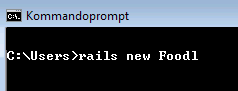
\includegraphics[scale=0.6]{billeder/Rails-new-foodl.png}
	\capt{Railskommando, der indtastes i kommandopromten, hvorefter rails genererer en mappe med en fuldtfungerende web-applikation, kaldet ``Foodl''}
	\label{fig:Rails-new-foodl}
\end{figure}

Enhver Railsapplikation tager udgangspunkt i arkitekturen Model-View-Controller. Mappen med webapplikationen består af en lang række undermapper, hvori ``models'', ``views'' og ``controllers'' bl.a. befinder sig. Kort sagt genererer Rails, vha. \texttt{new}-kommandoen, hele skelettet for webapplikationen, og derefter er det ``bare'' at fylde det indhold, man ønsker i sin webapplikation, i de rigtige mapper. Denne Model-View-Controllerarkitektur vil blive forklaret yderligere i følgende \secref{subsec:mvc}.

\subsection{Model-View-Controller}
\label{subsec:mvc}
3-lag arkitekturen minder meget om Model-View-Controller mønstret, som vi benytter og har kort beskrevet i \secref{subsec:mvc}. Dog skal det nævnes, at de ikke er helt ens. I en 3-lags komponentarkitektur er det ikke muligt for præsentationslaget at tilgå modellen. MVC-mønstøret er mere trekantet idet, at views kan tilgå både funktionskomponenten og modelkomponenten og dermed blive opdateret direkte fra modellen\cite{designpatterns}. MVC-arkitekturen kan ses i \figref{fig:komponenter}. Der findes mange forskellige frameworks, der bygger på MVC-arkitekturen. Fordelen er ved at benytte et eksisterende og anerkendt framework, er dets mange funktioner og brugervenlighed, der gør det muligt at hurtigt kunne implementere de nødvendige dele af systemet.

Arkitekturen består af tre hovedkomponenter: model, view og controller. Modelkomponenten bærer de data, som typisk er repræsenteret som tabeller i en database, der skal kunne manipuleres. Controllerkomponenten fungerer som et slags bindeled mellem modellen og views ved at sende forespørgsler til modellen eller views, alt afhængig af brugerinputtet fra de tilsluttede views. Derudover sender controlleren også forespørgsler i form af tilstandsændringer til modellen, hvis brugeren \fx opdaterer noget i et view. Et view præsenterer brugeren for data i modellen og muliggør ændringer i tilstanden af modellen.

Vi benytter også klient-server arkitekturmønstret, se \figref{railsmvc} der er oplagt, netop fordi vores model består af rigtig mange opskrifter. Det vil være upraktisk at overføre alle opskrifterne til hver eneste bruger, der benytter systemet, da det vil give en stor belastning på systemet og stor ventetid for brugeren. Vi lader derfor webbrowserkomponenten fungere som klient og tilkobler sig serveren under for at sende forespørgsler. Det er controller-komponenten, der sørger for at sende data frem og tilbage mellem klienten og server. Der er altså kun én server, som integrerer med mange forskellige klienter igennem et netværk og deler fælles ressourcer med alle de klienter, der er tilkoblet. Serverkomponenten stiller diverse funktioner tilgængelig for klienterne, \fx at muliggøre søgning eller lagring af oplysninger i modelkomponenten. Serveren, i dette tilfælde, og i modsætning til klient-servermønstret beskrevet i OOA\&D\cite{ooad}, kan godt kende noget til/om klienten. \Fx er det muligt, at vise andre views, alt afhængigt af hvilken webbrowser, der bliver tilkoblet serverkomponenten.

\pdffig[0.7]{railsMVC}{Et tilpasset generiske Model-View-Controller mønster indkapslet i et klient-server arkitekturmønster\cite{railsmvc}.}{fig:railsmvc}


\section{Brugergrænseflade}
\label{sec:webapplikationen}
Vi har udviklet en webapplikation, som vi har valgt at kalde \Foodl. I dette afsnit bliver webapplikationen præsenteret og beskrevet.

Vi har valgt at gøre designet så enkelt som muligt for ikke at forvirre brugerne. Når man kommer taster sig ind på hjemmesiden \url{http://www.foodl.dk}, bliver man mødt af en velkomsthilsen, der meget kort beskriver hjemmesidens formål og brug. Denne hilsen kan bruge vælge at lukke ned. En cookie bliver gemt i browseren, så velkomsthilsnen ikke bliver vist igen, medmindre browserhistorikken bliver ryddet.

Figur \ref{fig:foodl-forside} viser forsiden af hjemmesiden, uden velkomsthilsnen. Navnet \Foodl er også en del af webapplikationens logo. For at gøre det mere klar for en ny bruger, hvad siden handler om, så har vi erstattet et O i navnet med en stor ananas, fordi det er noget, der kan spises, og sidens formål er at give folk mulighed for at genbruge deres madrester. 

\begin{figure}[H]
	\centering
	
\includegraphics[scale=0.7]{billeder/foodl/forside.jpg}
	\capt{Denne figur viser webapplikationens startside. Logoet med den store ananas, der skal forestille bogstavet O, har til formål at byde brugerne velkomne til siden. Direkte under logoet kan brugerne indtaste de råvarer, de ønsker at bruge til madlavningen.}
	\label{fig:foodl-forside}
\end{figure}

På alle undersider af \url{foodl.dk} er det muligt at tilgå sidehovedet. Her er der mulighed for at navigere tilbage til forsiden ved at klikke på den mindre version af det store logo, som blev vist på forsiden. Derudover kan man tilgå både en indkøbsliste og en liste af favorit-opskrifter, som brugeren selv vælger fra hjemmesiden. Både indkøbslisten og favoritter har et tal i parentes, der \fx fortæller brugeren, hvor mange varer, der er i den nuværende indkøbsliste eller hvor mange opskrifter, der er gemt under favoritter. Dette kan ses på \figref{fig:foodl-header}.

Ydermere kan man se på \figref{fig:foodl-header}, at det er muligt at logge ind eller oprette en bruger i webapplikationen. Dette er dog ikke obligatorisk, da vi ikke ønsker at binde brugerne til at oprette noget som helst. Man kan bruge systemet, om man har en bruger eller ej. Den eneste fordel ved at oprette en bruger er, at man på denne måde kan gemme indkøbslisten og favoritterne under hver bruger til fremtidigt brug.

\begin{figure}[H]
	\centering
	
\includegraphics[scale=0.7]{billeder/foodl/header.jpg}
	\capt{Denne figur viser webapplikationens sidehoved, hvilket kan ses på alle undersider. Herfra kan forsiden (foodl), indkøbslisten og favoritter tilgås. Derudover er der mulighed for at brugeren kan logge ind eller oprette en bruger. Dette er frivilligt. Systemet kan godt bruges uden at oprette en bruger.}
	\label{fig:foodl-header}
\end{figure}

Som sagt så har brugeren ikke behov for at logge ind for at bruge systemet. Det er nu op til brugeren at indtaste alle de råvarer, der ønskes brugt til madlavningen. Figur \ref{fig:foodl-soegefelt} viser, hvordan en sådan søgning foregår. Der bliver løbende indtastet bogstaver, og systemet undersøger for dele af tekststrenge, der matcher det der bliver indtastet. Ud fra disse match gives der forslag til hvilke råvarer, man kan vælge. Man kan ikke indtaste hvad som helst som et søgekriterie i systemet. Der er en lang række råvarer at vælge imellem. Hvis der \fx bliver indtastet kød i søgefeltet, så kommer der en liste af matchende råvarer som forslag, som man kan se på \figref{fig:foodl-soegefelt}.

For at fuldføre en søgning skal man blot trykke på ``Søg'', der er til højre for søgefeltet. Når brugeren trykker ``Søg'', så arbejder systemet på at finde alle de opskrifter, der minimum har en ingrediens, der matcher en af de indtastede råvarer.

\begin{figure}[H]
	\centering
	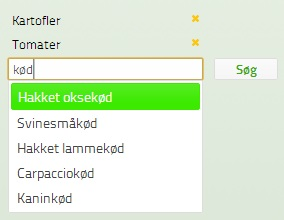
\includegraphics[scale=0.7]{billeder/foodl/soegefelt.jpg}
	\capt{Denne figur viser webapplikationens søgefelt. Når brugeren begynder at stave til de råvarer, der ønskes at blive brugt i madlavningen, så giver webapplikationen forslag til råvarer, der er søgbare i systemet, som indeholder lignende tekst-dele, hvilket brugeren løbende bliver indtaster i feltet. Der er også mulighed for at slette valgte råvarer ved at trykke på de små gule krydser ud for råvaren. Når brugeren har valgt alle de råvarer, der ønskes brugt, så skal brugeren trykke på Søg-knappen for at fuldføre søgningen.}
	\label{fig:foodl-soegefelt}
\end{figure}

Det er efter denne søgning, at brugeren finder ud af, hvad der er muligt at lave ud fra de råvarer, der er til rådighed. Resultatet er selvfølgelig afgrænset til den database man har over opskrifter.

Når søgningsresultatet vises, så er det en liste af opskrifter. I første omgang er opskrifterne sorteret efter relevans, dvs. hvor mange ingredienser, der matcher de forskellige indtastede råvarer. Figur \ref{fig:foodl-opskrift} viser et eksempel af en opskrift, der er et resultat af den foretagede søgning. I eksemplet er der kun 1 ingrediens, der matcher de indtastede råvarer, og denne er markeret med fed skrift (semidried tomatoes).

På hjemmesiden vises der kun hvilke ingredienser, der skal til for at lave opskriften, men selve fremgangsmåden er ikke vist nogen steder. Man er nødt til at tilgå den oprindelige hjemmeside, hvorfra opskriften stammer fra. Dette gøres ved at trykke på enten opskriftens titel eller billedet. Begge elementer består af et link til opskriftens originale hjemmeside. 

Fremgangsmåden kan ikke ses på vores hjemmeside, men alle andre vigtige elementer af opskriften er synlige. En opskrift består af følgende elementer:

\begin{itemize}[noitemsep]
\item Titel
\item Billede
\item Tilberedningstid
\item Relevans (antal matchende ingredienser)
\item Ingredienser
\item Knapper
\begin{itemize}[noitemsep]
\item Tilføj alle ingredienser til indkøbsliste
\item Tilføj / fjern fra favoritter
\item Tilføj enkelte ingredienser til indkøbsliste
\item Indmeld en fejl med opskriften
\end{itemize}
\end{itemize}

Alle opskrifter består af en beskrivende titel og et relevant billede, der skal vise brugeren, hvordan opskriften kan se. Billedet er med til at vække en interesse hos brugeren. Tilberedningstiden er også en vigtig ting at være klar over, og denne kommer direkte under billedet. De matchende ingredienser er markeret med fed skrift, så har brugeren nemmere ved at gennemskue, hvad der \fx er relevant at handle ind ud fra alle ingredienserne. Derudover er der et sæt knapper, som brugeren kan bruge. Se \figref{fig:foodl-opskrift}. I øverste højre hjørne er der en knap, der har et notesblok-lignende ikon. Denne knap tilføjer alle ingredienserne til indkøbslisten. Der er også mulighed for at tilføje de enkelte ingredienser ved at trykke på de små plus'er ud for ingredienserne. Ydermere er der mulighed for at tilføje og fjerne en opskrift til ens favorit-liste. Dette gøres ved at trykke på den hjerte-formede knap. I nederste højre hjørne er der en advarselsknap, der bruges til at rapportere om eventuelle fejl ved den specifikke opskrift.

\begin{figure}[H]
	\centering
	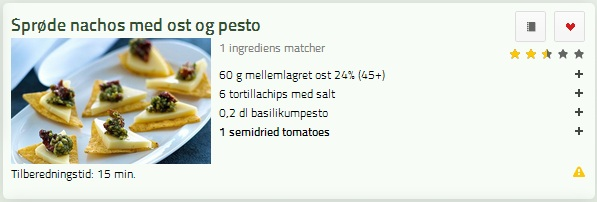
\includegraphics[scale=0.7]{billeder/foodl/opskrift.jpg}
	\capt{Når brugeren fuldfører en søgning, så bliver brugeren præsenteret med en liste af opskrifter, der minimum indeholder en ingrediens, der passer med en af de råvarer, som blev indtastet af brugeren. Her ses en opskrift ud af en liste af opskrifter, som var resultatet af søgningen, der blev foretaget. Et søgeresultat består af opskriftens titel og billede, hvilket begge er link, der fører brugeren videre til opskriftens fremgangsmåde på dens originale hjemmeside. Direkte under billedet kan man se, hvor lang tid det ca. tager at tilberede opskriften. Derudover kan man se, hvor mange ingredienser, der matcher fra søgningen, og de ingredienser, der matcher er markeret med fed skrift i resultatet. I øverste højre hjørne af resultatet, kan man (ved den hjerteformede knap) tilføje og fjerne en opskrift fra favoritter. Knappen til venstre for hjertet, der er formet som en lille notesblok, tilføjer alle ingredienserne til brugerens indkøbsliste. Direkte under disse to knapper kan man se,hvor mange stjerner en opskrift har fået. Opskrifterne får stjerne ud fra det antal brugere, der har favoriseret opskriften. De små plusser bruges til at tilføje enkelte ingredienser til indkøbslisten. I nederste højre hjørne er der en advarselsknap, som bruges til rapportering af eventuelle fejl med den specifikke opskrift.}
	\label{fig:foodl-opskrift}
\end{figure}

Brugeren har forskellige muligheder for at manipulere søgningsresultatet. Der er blevet implementeret en toolbar i toppen af siden, der følger brugerens bevægelser mht. at scrolle op og ned. På denne måde behøver brugeren ikke at scrolle helt til toppen for at udføre en handling på søgningsresultatet. 

Figur \ref{fig:foodl-toolbar} illustrerer, hvordan toolbaren ser ud. I venstre side er der en samling af tre knapper, der bruges til at begrænse søgningsresultatet mht. tilberedningstiden. Her er der mulighed for at markere flere af gangen, og default kriteriet er, hvis ingen er markeret, så er alle markeret. Dette betyder, at systemet starter med at vise alle resultater. I midten af toolbaren er der et skaleringsværktøj, der kan bruges til at skalere opskrifternes portioner mht. antal personer. Man kan skalere dem ned til 1 person og op til 10 personer. Vi valgte 10 som maximum, fordi det er relativt let at skalere yderligere, hvis dette er ønsket. Til højre er der endnu en samling af tre knapper, men disse benyttes til at sortere opskrifterne. Default er relevans. De to knappesamlinger er forskellige på to måder; hvad de bruges til, og at der kun er mulighed for at markere en knap af gangen ved sorteringsknapperne (højre side) og mulighed for markering af flere af gangen ved afgrænsningsknapperne (venstre side).

\begin{figure}[H]
	\centering
	
\includegraphics[scale=0.7]{billeder/foodl/toolbar.jpg}
	\capt{Toolbaren er direkte under sidehovedet. I venstre side af toolbaren er der en samling af tre knapper, der kan specificere en søgning ud fra tilberedningstiden. I midten af toolbaren kan man skalere opskrifterne fra 1 til 10 personer. Til højre kan man sortere listen af opskrifter efter navn, relevans eller tilberedningstid. Toolbaren følger vinduet, når man scroller op og ned, så brugeren altid kan manipulere listen af opskrifter efter behov.}
	\label{fig:foodl-toolbar}
\end{figure}

Ud over toolbaren, så viser \figref{fig:foodl-sidebar} en sidebar, hvilket gør det mulight for brugeren at følge med i, hvad der bliver søgt på, og den er en mulighed for brugeren at lave endnu en søgning. Man kan herfra slette og/eller tilføje nye råvarer til en ny søgnign. Denne sidebar følger også brugeres scrolling, da det skal være nemt og hurtigt at lave en ny søgning, hvis dette bliver aktuelt.

\begin{figure}[H]
	\centering
	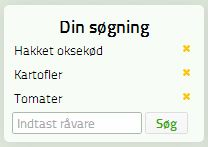
\includegraphics[scale=0.7]{billeder/foodl/sidebar.jpg}
	\capt{Sidebaren er placeret venstre for listen af opskrifter, og bruges til at holde brugeren opdateret med, hvilke råvarer, der er blevet søgt på. Man kan direkte fra denne redigere søgningen og udføre en ny søgning. Sidebaren følger vinduet, når man scroller op og ned, så brugeren altid er klar til at søge igen.}
	\label{fig:foodl-sidebar}
\end{figure}

Hvis en bruger vælger at benytte sig af indkøbslisten, så kan denne tilgås via sidehovedet, som kan ses på \figref{fig:foodl-header}, ved at trykke på ``indkøbsliste''. I sidehovedet kan man også se, hvor mange varer, der er blevet tilføjet til listen. 

Man kan tilføje hvilken som helst tekststreng til indkøbslisten. På denne måde har vi ikke begrænset brugeren til blot at tilføje ingredienser fra opskrifterne, men det er helt op til brugeren selv at bestemme, hvad skal på listen. Brugeren har mulighed for at tilføje varer i feltet ``tilføj til indkøbsliste'' og trykke på ``tilføj''. Der er mulighed for at slette alle varer fra indkøbslisten og ligeledes at slette enkelte varer. Derudover er der implementeret en knap, til at udskrive indkøbslisten, hvis det skulle være nødvendigt.

\begin{figure}[H]
	\centering
	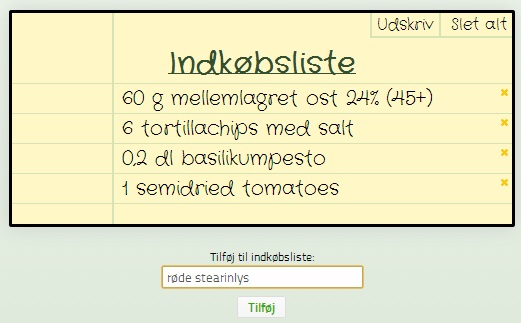
\includegraphics[scale=0.7]{billeder/foodl/indkoebsliste.jpg}
	\capt{Indkøbslisten tilgås fra sidehovedet. Her får brugeren mulighed for at se, hvad der er blevet tilføjet til indkøbslisten og eventuelt tilføje flere varer. I dette eksempel ønskes der at tilføjes røde stearinlys til listen. Brugeren har mulighed for at slette alle varer på listen ved at trykke på knappen i øverste højre hjørne, eller brugeren kan slette enkelte varer, der ikke skal købes. Derudover er der mulighed for at udskrive listen ved at klikke på knappen i øverste højre hjørne.}
	\label{fig:foodl-indkoebsliste}
\end{figure}

I \figref{fig:foodl-opskrift} vises en knap, der bruges til at rapportere eventuelle fejl ved de specifikke opskrifter. Figur \ref{fig:foodl-fejlrapportering} viser, hvordan det ser ud, når en bruger trykker på rapporteringsknappen ved en opskrift. Der popper en lille boks op, og baggrunden af siden bliver mørk. Her kan man nu specificere, hvad fejlen handler om og give en beskrivelse, inden man vælger at indsende fejlen.

\begin{figure}[H]
	\centering
	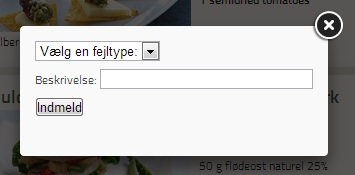
\includegraphics[scale=0.7]{billeder/foodl/fejlrapportering.jpg}
	\capt{Når en bruger opdager en fejl ved en opskrift, så har brugeren muligheden for at indberette fejlen ved at trykke på advarselsknappen, der kan ses i \figref{fig:foodl-opskrift}. Brugeren kan nu vælge en fejltype og beskrive dennne, inden fejlen bliver indmeldt.}
	\label{fig:foodl-fejlrapportering}
\end{figure}

Muligheden for oprettelse af bruger er tilstede. Figur \ref{fig:foodl-opret} viser, hvordan denne ``log ind / opret bruger'' side ser ud. Man skal bruge sin email og en adgangskode for at lave en bruger. Hvis man allerede har en bruger, så skal man blot logge ind med de rigtige oplysninger. Som det tidligere blev nævnt, så er det ikke obligatorisk at oprette en bruger. Den eneste fordel der er ved dette er, at man får mulighed for at gemme indkøbslisten og listen over favoritter. 

Når man er logget ind, så ændrer sidehovedet sig en smule. Figur \ref{fig:foodl-header-loggetind} viser, at der nu er mulighed for at gå ind i en menu, der hedder ``indstillinger'' og at logge ud igen. Man kan også se, at der pludselig er indlæst en liste af favoritter på 10 opskrifter fra tidligere besøg.

\begin{figure}[H]
	\centering
	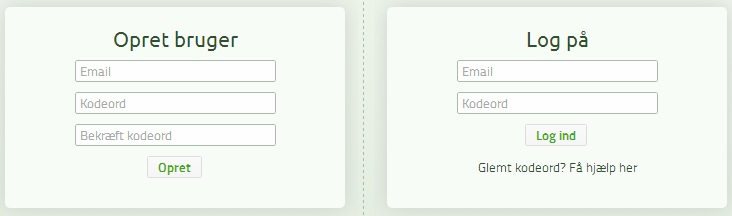
\includegraphics[scale=0.7]{billeder/foodl/login-opret.jpg}
	\capt{Hvis brugeren ønsker der, så kan man oprette en bruger i webapplikationen. Dette gør det muligt at gemme favoriseringer og indkøbsliten til brug i fremtiden eller på andre enheder. Når man trykker på ``log ind / opret bruger'', som kan ses i \figref{fig:foodl-header}, bliver brugeren præsenteret med to valg. Muligheden for at logge ind eller oprette en bruger. Her skal der indtastes e-mail og adgangskode.}
	\label{fig:foodl-opret}
\end{figure}

\begin{figure}[H]
	\centering
	
\includegraphics[scale=0.7]{billeder/foodl/header-login.jpg}
	\capt{Når brugeren er logget ind, så ændrer sidehovedet sig en smule. ``log ind / opret bruger'' bliver erstattet med ``indstillinger'' og ``log ud''. Derudover indlæses eventuelle gemte favoritter og indkøbsliste.}
	\label{fig:foodl-loggetind}
\end{figure}

Hvis man ønsker at skifte sin adgangskode, så sker det ved at trykke på knappen ``indstillinger'' i sidehovedet. Dette illustrerer \figref{fig:foodl-indstillinger}.

\begin{figure}[H]
	\centering
	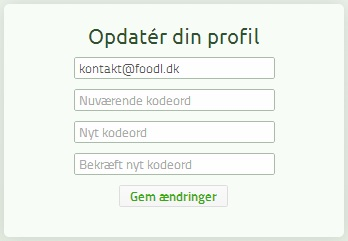
\includegraphics[scale=0.7]{billeder/foodl/indstillinger.jpg}
	\capt{Brugeren har mulighed for at ændre nogle basale indstillinger ved at klikke på ``indstillinger'' i sidehovedet, som kan ses i \figref{fig:foodl-loggetind}. Her kan brugeren ændre sin adgangskode.}
	\label{fig:foodl-indstillinger}
\end{figure}

Som de fleste andre hjemmesider, så har vi også en ``om'' og en ``kontakt'' side, som kan tilgås fra nederste venstre hjørne af enhver foodl-underside. Derudover kan man rapportere en generel fejl ved siden, hvis man støder på sådan en.

\begin{figure}[H]
	\centering
	
\includegraphics[scale=0.7]{billeder/foodl/formaliteter.jpg}
	\capt{I nederste venstre hjørne af webapplikationen kan man rapportere en generel fejl, læse mere om webapplikationen og kontakte udviklerne.}
	\label{fig:foodl-formaliteter}
\end{figure}

\subsection{Parsing af Opskrifter}
Opskrifterne på Arla blev parset ved brug af modulet Nokogiri i Ruby. Nokogiri-modulet gør det let at finde værdier af forskellige elementer i et dokument. På Arlas hjemmeside findes en side, der giver mulighed for at vise alle opskrifterne. Der vises 16 opskrifter af gangen, og når man bladrer frem og tilbage imellem side 1 og side 2, hver især med 16 forskellige opskrifter på hver, så ændres en query i url'en på følgende måde: \\
\lstinline{?...\&paging=1\&...} \\
\lstinline{?...\&paging=1\&...} \\
En variabel ved navn \textit{paging} ændres i queryen værdi fra 1 til 2. Siderne, der indekserer 16 opskrifter af gangen er derfor lette at finde ved blot at lade en variable gå fra 1 og øges indtil ingen opskrifter fremkommer.

På hver enkelt indekseringsside vises 16 opskrifter. Et link til en opskrift på Arlas indekseringsside, ser i HTML således ud:

\lstinline{<h2><a href="/opskrifter/Suppe">Suppe</a></h2>}

Ved at bruge klassen \textit{xpath} i Nokogiri, kan alle 16 links hurtigt returneres som at array ved at benytte funktionen:

\texttt{xpath("//h2//a").map{|link| "http://www.arla.dk"+link["href"]}}

Metoden \textit{xpath}, leder efter alle \textit{<a>} tags inde i \textit{<h2>} tags og returnerer et array af elementer, der hver især har en værdi for indekset \textit{href}, der svarer til linket til siden. Ved at bruge funktionen \textit{map}, fås værdien af indekset \textit{href}, og præfixet \texttt{http://www.arla.dk} tilføjes foran. En forudsætning, der var til stede, for at kunne benytte denne metode, var at samme tagsekvens, i dette tilfælde \lstinline{<h2><a>}, ikke blev benyttet til andet end de links vi var interesserede i.

Med en mulighed for at finde alle opskrifters unikke url, begyndte vi at undersøge opbygningen af siden der viser en enkelt opskrift.
På samme måde kunne Nokogiri også bruges her til at finde informationer omkring tilberedningstid, opskriftens navn, billede af opskriften og portionsstørrelse. Alle disse ting kunne indsættes som en ny række i databasens tabel `recipes`. Opskriftens navn vær særlig let at parse, da det var sidens titel, og kunne derfor tages fra HTML-tagget \textit{<title>}. Der var dog tilføjet lidt mere information, adskilt af karakteren ``|''. Et eksempel: \textit{Opskrifts navn | Kløver® | Produkter |}. Ved at bruge funktionen \textit{split} på karakteren ``|'', blev de forskellige dele, der var adskilt af ´´|'' hver især til ét element i et array. Opskriftens navn blev så det første element i arrayet.

Ingredienserne i en opskrift var nemme at parse, men hvordan de parsede ingredienser skulle håndteres vil nu blive forklaret.


\subsection{Parsing af ingredienser}

\subsubsection{Råvaretabellen}
\label{subsec:parsingafraavarer}
Efter afprøvning af prototyperne 2A og 2B på informanterne blev vi klar over at råvarer skal indtastes på forsiden i et design meget lig med Googles. Informanterne var glade for autocomplete-funktionen, der gør det muligt at indtaste teksten \textit{ba} i søge feltet og få stillet nogle forslag som \fx \textit{banan, balsamico}, så det ikke er nødvendigt at stave hele råvaren.
En autocomplete-funktion skal have noget data at stille forslag fra, og i dette tilfælde har vi brug for en tabel med alle de forskellige råvarer man kan forestille sig at en bruger vil indtaste. Denne tabel over råvarer vil fremover blive kaldt råvaretabellen.

Da opskrifterne, der søges på, kommer fra Arla, ville det have været nemt hvis Arla havde offentliggjort en liste over de forskellige ingredienser de benytter, således vi kunne bruge denne data som vores råvaretabel. En sådan liste var ikke til at finde, så vi begyndte at overveje muligheden for at lave råvaretabellen ved at parse ingredienserne direkte fra Arlas opskrifter. Et eksempel på ingrediensernes navne i Arlas opskrifter:

375 g rød peberfrugt i strimler

3 røde peberfrugter (ca. 600 g)

4 røde peberfrugter i store tern (ca. 500 g)

En bruger, der indtaster teksten \textit{pe} i forsøget på at indtaste \textit{rød peberfrugt}, skal kun præsenteres for forskellige råvarer, og altså ikke samme råvare i forskellige mængder og former (skiver, strimler, hakket, m.m.). Det vil sige, at de mange forskellige ingredienser, der alle består af en rød peberfrugt, kun skal medføre at \textit{rød peberfrugt} findes én gang i råvaretabellen. Vi vurderede at Arlas navngivning af ingredienser har været for forskellig til blive brugt som kilde til vores råvaretabel. Råvaretabellen er i stedet blevet lavet ud fra en liste af råvarer offentliggjort af madopskrifter. Et udpluk af listen ser således ud:

\begin{itemize}
\item Rød peberfrugt
\item Persille
\item Citron
\end{itemize}

Listen fra madopskrifter.nu blev brugt som vores råvaretabel af følgende grunde:

\begin{itemize}
\item Listen indeholdt kun 4 dubletter, som blev fjernet
\item Råvarerne indeholdt kun den rå råvare, ingen mængder eller andre betegnelser (vaskede, skrællede, m.m.)
\item Listen omfattede 933 råvarer, hvilket vi anså som rigeligt
\end{itemize}

\subsubsection{Parsing af opskrifter}
Råvaretabellen giver brugeren mulighed for at indtaste en mængde råvarer. Hvis han indtaster råvaren \textit{gulerødder}, skal han have muligheden for at udføre en søgning, der finder alle opskrifter, der indeholder gulerødder. Det er derfor nødvendigt, ud fra alle ingredienser i en opskrift, at kunne afgøre hvilken af råvarerne i råvaretabellen, der er magen til. Som før nævnt er ingrediensernes navne i Arlas opskrifter meget inkonsistente. Derfor vil navnene kun i få tilfælde være helt ens. Det er derfor nødvendigt med en metode til at kunne sammenligne to tekster og bestemme hvor meget de minder om hinanden. Med en sådan metode vil det nemlig være muligt, for hver ingrediens at finde den råvare der minder mest om. Dette begreb vil i afsnittet blive kaldt for mapping. Metoden, vi bruger til at sammenligne to tekststrenge for lighed, vil vi fremover kalde \textit{CompareStrings}.

Hvis \textit{CompareStrings} køres hver gang der udføres en søgning, vil det stille høje krav til hastigheden af denne funktion, for at brugeren kan udføre en hurtig søgning. For ikke at sætte krav til hastigheden af funktionen, benytter vi en relationstabel. For hver opskrift fundet på Arla sammenligning vi hver enkelt ingrediens i opskriften med alle råvarerne i råvaretabellen med vores \textit{CompareStrings}. For hver ingrediens indsættes én relation mellem ingrediensen og den råvare i råvaretabellen, som ingrediensen bedst matcher ifølge vores \textit{CompareStrings}. Når en bruger udfører en søgning, vil \textit{CompareStrings} slet ikke blive benyttet. Det vil kun være nødvendigt at undersøge de indtastede råvares relationer til ingredienser, og blot præsentere de opskrifter, der er relateret til de fundne ingredienser, som et søgeresultat for brugeren.


\subsubsection{Sammenligning af 2 tekststrenge}
Der findes mange forskellige algoritmer til at sammenligne to tekststrenge for lighed. Det er vigtigt for os at finde en god og brugbar metode, der så korrekt som muligt kan mappe alle ingredienserne i Arlas opskrifter over til en passende råvare i vores råvaretabel. Det er ikke realistisk at opnå en 100 \% korrekt mapping. Vi har erfaret, at der nemt kan opstå problemer omkring ingredienser der minder meget om hinanden, som \fx ved mapping af ingrediensen \textit{hakket løg}. En parser vil have svært ved at vide, at \textit{hakket løg} skal mappes til råvaren \textit{løg} og ikke \textit{hakket oksekød}. En korrekt mapping vil i dette tilfælde kræve kendskab til at ordet \textit{hakket} er et udsagnsord og derfor bør fjernes før der forsøges at mappe. Men hvis vi vil mappe ingrediensen \textit{hakket oksekød}, så er det nødvendigt at ordet \textit{hakket} stadig indgår under mappingen (på trods af at det er et udsagnsord), fordi der findes mange former for oksekød og vi ønsker at skelne imellem de forskellige former.

Vi har brugt tilfældigt udvalgte ingredienser fra Arlas opskrifter til at teste 5 forskellige metoder til tekstsammenligning. I mange tilfælde kunne alle 5 metoder mappe en ingrediens til en korrekt råvare. I enkelte tilfælde skete der dog en fejlmapping, hvilket kan ses i \tableref{table:mapping}.

\paragraph{Forklaring af de forskellige \textit{CompareStrings} funktioner}
\begin{enumerate}
\item Egen algoritme (lineær)
\item Egen algoritme (polynomial)
\item Levenshtein (1 point for slet, tilføj og udskift) %kilde ruby gem levenshtein.distance
\item Levenshtein (1 point for slet, tilføj og udskift. Score divideres med længste streng) %kilde ruby gem levenshtein.normalized_distance
\item Levenshtein (1 point for slet og tilføj. 2 point for udskift) %kilde ruby gem text.levenshtein.distance med modificeret vægt
\end{enumerate}


\begin{table}
    \begin{tabular}{|p{2cm}|c|c|c|c|c|}
        \hline
        Ingrediens                                                 & Metode 1        & Metode 2                & Metode 3           & Metode 4           & Metode 5        \\ \hline
        dildkvist                                                  & \textbf{dild}            & \textbf{dild}                    & \textbf{dild}               & sildefilet         & dild            \\ \hline
        groft salt                                                 & \textbf{salt}            & citron saft             & frugtsaft          & frugtsaft          & \textbf{salt}            \\ \hline
        grofthakkede krydderurter, fx koriander, persille og dild & \textbf{krydderurtemix}  & \textbf{tikka (indisk krydderi)} & hakkede tomater    & hakkede tomater    & hakkede tomater \\ \hline
        basmatiris eller luftige urteris                           & \textbf{basmati ris}     & herbamare urtebouillon  & \textbf{basmati ris}        & \textbf{basmati ris}        & \textbf{basmati ris}     \\ \hline
        ostindisk karry                                            & \textbf{karrypasta}      & kinaradise              & sød sherry         & sød sherry         & \textbf{karry}           \\ \hline
        frisk salvie                                               & \textbf{salvie}          & \textbf{salvie}                  & fiskesauce         & fiskesauce         & \textbf{salvie}          \\ \hline
        koncentreret tomatpure                                     & \textbf{tomatpure}       & \textbf{tomatpure}               & soltørrede tomater & soltørrede tomater & \textbf{tomatpure}       \\ \hline
        hakket svinelever                                          & hakket svinekød & \textbf{svinelever}              & hakket svinekød    & hakket svinekød    & \textbf{svinelever}      \\ \hline
        store kapers med stilk                                     & \textbf{kapers}          & syltede artiskokhjerter & trefarvet is       & trefarvet is       & \textbf{kapers}          \\ \hline
        hvidvin fx rieslin                                         & \textbf{hvidvin}         & \textbf{hvidvin}                 & hvidvinseddike     & hvidvinseddike     & \textbf{hvidvin}         \\ \hline
        friskpresset limesaft                                      & \textbf{limesaft}        & \textbf{limesaft}                & appelsinsaft       & appelsinsaft       & \textbf{limesaft}        \\ \hline
        kartoffel                                                  & \textbf{kartofler}       & \textbf{kartofler}               & \textbf{kartofler}          & \textbf{kartofler}          & kartoffelmel    \\ \hline
        ~                                                          & ~               & ~                       & ~                  & ~                  & ~               \\ \hline
        Total:                                                     & 11              & 7                       & 3                  & 2                  & 10              \\
        \hline
    \end{tabular}
  \caption{Test af flere forskellige CompareStrings brugt til at mappe en ingrediens til en råvare. Fed skrift betyder at begge vores informanter har godkendt mappingen.}  \label{table:test-af-compares}
\end{table}

Som det ses i \tableref{table:test-af-compares}, var metode 1 den, der gav den bedste mapping. Metoden fik 11 rigtige ud af 12 mulige, men det bør bemærkes at sammenligningen kun er foretaget på de ingredienser, som mindst én metode mappede forkert. Vi kom forbi 56 ingredienser udover de ingredienser vist i tabellen, før vi tilsammen havde 12 ingredienser, som én eller flere metoder mappede forkert. 

Metode 1 er en algoritme vi selv har udviklet, der er beskrevet med pseudokode i \algref{alg:compare}. Den tager to tekststrenge som input, og returnerer en værdi mellem 0 og 100. Højere returværdi betyder større lighed mellem de to inputtede strenge. 100 point opnås kun ved to identiske strenge.
I \tableref{table:vores-compare-eksempel} ses et eksempel på hvordan algoritmen sammenligner \textit{hummersuppe} med \textit{suppe med hummerhale} og kommer frem til resultatet $13.8$.

\begin{table}
    \begin{tabular}{|l|l|l|}
        \hline
        str1        & str2                  & ~                             \\ \hline
hummersuppe & suppe med hummerhaler & $max\_length = 21$               \\         
        \textbf{hummer}suppe & suppe med \textbf{hummer}haler & $score = 6^2 = 36$               \\ 
        \textbf{suppe}       & \textbf{suppe} med haler       & $score = score + 5^2 = 36 + 25 = 61$                 \\ 
        ~           &  med haler            & $no common substrings found$        \\ 
        ~           & ~                     & $max\_score = 21^2  = 441$    \\ 
        ~           & ~                     & $return \frac{61 \times 100}{441} = 13.8$ \\
        \hline
    \end{tabular}
    \caption{Her vises et eksempel på hvordan vores algoritme sammenligner \textit{hummersuppe} med \textit{suppe med hummerhaler}.}
    \label{table:vores-compare-eksempel}
\end{table}

Metode 2 var magen til metode 1, bortset fra at scoren blev forøget lineært i stedet for opløftet i anden. Se linje 7, \algref{alg:compare}. På samme måde blev variablen $max\_score$ i linje 5 også beregnet lineært.

\begin{algorithm} [H]
	\capt{Algoritmen udregner hvor ens to tekststrenge er.}
	\label{alg:compare}
	\input{pseudokode/parsing}
\end{algorithm}



\subsubsection{Mapping af ingredienser til råvarer}
Den automatiske mapping omfattede 10,234 ingredienser, blandt 921 opskrifter. Tidsforbruget var ca. 4 timer, og langt de fleste ingredienser blev mappet korrekt. Ind i mellem gik mappingen galt, fx. blev ingrediensen \textit{groftkværnet peber} hver gang mappet til råvaren \textit{hvid peber} i stedet for råvaren \textit{peber}. For at få en bedst muligt mapping besluttede vi os for at gå alle mappings igennem igennem manuelt. Under mappingen havde vi gemt returværdien af \textit{CompareStrings(string, string)}, der fortæller hvor ens de to sammenlignede tekstrenge var. Ved at have gemt returværdien behøver vi ikke at kontrollere mappings, der har returneret 100, da det vil sige at ingrediensen er blevet mappet til en identisk råvare. På denne måde kunne vi se bort fra 1,236 ingredienser, der ikke behøvede manuel kontrol.
Til at mappe ingredienserne hurtigst muligt lavede vi et meget simpelt WinForms program med Visual Studio, skrevet i C\# (se \apref{ap:manuel-mapping}. Programmet gjorde det muligt at få vist 20 labels med ignredienser. Ud for hvert label blev vist et tekstfelt med den råvare, som ingrediensen var blevet mappet til. Ved at ændre i tekstfeltet kunne man hurtigt få lavet en korrekt mapping. Vi tilføjede flere funktionaliteter for at øge hastigheden vi kunne mappe med.
\begin{itemize}
\item Ingredienserne blev sorteret alfabetisk. Omkring 120 ingredienser i træk var \textit{grofthakket peber}.
\item Autocomplete gjorde det nemt at se hvilke råvarer man kunne vælge imellem og også hurtigere at indtaste råvaren.
\item Råvarer kunne tilføjes hvis ingen fandtes, der matchede en given ingrediens.
\item Ingredienser som \fx \textit{grillspyd} og \textit{lagkageflag} kunne fjernes i programmet.
\item En hel side kunne godkendes med ét klik, hvis alt var mappet korrekt på forhånd.
\end{itemize}

Tidsforbruget på remappingen var ca. 6 mandetimer, hvilket kan omregnes til $\frac{10234 - 1236}{6} = 1500$ ingredienser pr. mandetime.
 	

\chapter{Kvalitetssikring}
\label{chap:kvalitetssikring}

\section{Afprøvning af prototype 1}

\paragraph{Mål}
Blandt 2 prototyper (1A og 1B), at udvælge den bedste metode til at finde og tilføje ingredienser, slette ingredienser, samt søge efter opskrifter med de valgte ingredienser.
Prototyperne er radikalt forskellige på dette område. Med prototype 1A vælges en ingrediens kun med musen. Dette gøres ved først at vælge en kategori, der muligvis bliver til en underkategori op til flere gange, og til sidst fås en liste af ingredienser indenfor den valgte kategori / underkategori, hvorfra en enkelt ingrediens nu kan vælges. Med prototype 1B vælges en ingrediens ved at indtaste dele af- eller hele navnet på ingrediensen i et søgefelt. Under indtastningen af navnet, kommer der løbende forslag til ingredienser, der starter med den indtastede tekststreng.
\begin{table}[H]
   \centering
    \begin{tabular}{|l|l|l|l|}
        \hline
        ~                    & \textbf{Fokus} & \textbf{Afgræsninger}              & \textbf{Forudsætninger}            \\ \hline
        \textbf{Grænseflade} & Forsiden       & Der fokuseres på, hvordan          & Brugeren kender formålet med siden \\
        ~                    & ~              & ingredienser findes og tilføjes    &                                    \\ \hline 
        \textbf{Funktioner}  & ~              & ~                                  & ~                                  \\  \hline
       \textbf{Model}        & ~              & ~                                  & ~                                  \\
        \hline
    \end{tabular}
    \capt{Hvad vides inden afprøvningen?}
    \label{table:afproevning1}
\end{table}	


\textbf{Opgaver til informant}

\textbf{For hver prototype:}
\begin{enumerate}[noitemsep]
\item Du ønsker at finde en opskrift, der indeholder både kylling, broccoli og ananas. Hvad gør du?
\item Du kommer i tanke om, at din ananas er alt for gammel, og ønsker at fjerne denne fra listen. Hvad gør du?
\end{enumerate} 

\textbf{Evaluering:}
\begin{enumerate}[noitemsep]
\item Hvilken prototype foretrak du? 
\end{enumerate}

\textbf{Afprøvning foretaget af informant Merete Munthe, 24 september, Gistrup:}
\tjek{Afprøvning kan ses på linket: kommer snart}

\textbf{Prototype 1A:}
\begin{enumerate}[noitemsep]
\item Informanten valgte at trykke søg hver eneste gang hun havde valgt en ingrediens. Altså vælg kylling, tryk søg, vælg broccoli, tryk søg og vælg ananas, tryk søg. Efter test af prototypen blev der for en sikkerheds skyld spurgt hvordan hun havde forstået opgaven. Hun havde forstået opgaven korrekt, nemlig at hun skulle søge efter de opskrifter, der indeholdt alle 3 ingredienser, og ikke foretage 3 forskellige søgninger på opskrifter indeholdende hver af disse 3 ingredienser.
\item Informanten slettede korrekt ananas ved at trykke på krydset.
\end{enumerate}

\textbf{Prototype 1B:}
\begin{enumerate}[noitemsep]
\item Informanten forstod at vælge ingredienserne korrekt, og trykkede først søg efter alle 3 ingredienser var korrekt valgt.
\item Informanten slettede korrekt ananas ved at trykke på krydset.
\end{enumerate}

\textbf{Evaluering}
Informanten foretrak prototype 1B, hvor man kan søge på ingredienser ved brug af tastaturet. Dette mente hun ville være hurtigere for hende, da hun ikke skulle tænke over hvilken kategori en ting ligger under, og valget af en ingrediens synes hun gik hurtigere med prototype 1B.
\chapter{Konklusion}
\label{chap:konklusion}





\cleardoublepage
	
\bibliographystyle{plain}
\bibliography{kildeliste}

\part{Akademisk rapport}


\part{Bilag}

\appendix
%\chapter{Appendiks Eksempel}
\label{ap:eksempel}

\chapter{Fravalgte klasser og hændelser}
\label{ap:fravalgteklasseroghændelser}

Herunder ses de fravalgte klasser, som gruppen ikke finder relevante i forhold til problemområdet. De listes her, da der har været meget diskussion, om hvorvidt klasserne skulle med i systemet eller ej. 

\begin{description}
\item[Person] \hfill \\
Vi vælger at fjerne person-klassen, fordi vi mener, at vores løsning ikke skal være noget socialt media, og derfor mener vi, at det er selve husholdningen, der er fælles om madlavningen selvom det måske blot er en person, der laver mad og står for indkøb og lignende. Brugeren af programmet er ikke en del af problemområdet og skal derfor ikke modelleres som klasse.

\item[Køkken] \hfill \\
Køkken og husholdning dækker over samme del af problemområdet, og vi fjerner derfor køkken og vurderer bagefter om husholdning skal være en klasse.

\item[Husholdning] \hfill \\
En husholdning repræsenterer et hjem, som indeholder én til flere personer. Det er ikke en del af problemområdet at holde styr på eller at kommunikere med andre husstande.

\item[Køleskab/skab/opbevaringsskab] \hfill \\
Om råvarene befinder sig i et køleskab eller i en skuffe er, for os, uinteressant, derfor er vi ikke interesseret i at modellere disse skabe som en klasse.

\item[Køkkenredskab/komfur] \hfill \\
Ligesom ved køleskab/anden opbevaring er vi ikke interesseret i at modellere hvilke redskaber husholdningen har adgang til.

\item[Service] \hfill \\ 
Vi har valgt at fjerne klassen service, fordi denne ikke findes i vores problemområde. Service er noget, der bliver brugt, når man er i færd med at spise det færdige mad, og ikke under selve madlavningen.

\item[Butik] \hfill \\
Vi har valgt at fjerne klassen Butik, da vores system fokuserer på madspild og varieret kost. En modellering af butikker ville være relevant, hvis vores fokus lå på at begrænse udgifter på mad, men da dette imidlertidig ikke er situationen i problemområdet, bliver den udeladt.

\item[Typisk/atypisk ingrediens] \hfill \\
Det er ikke en del af problemområdet at folk ikke er klar over hvilke ingredienser der er normale/unormale at have.

\item[Enhed/Mængde] \hfill \\
Enhed og mængde er ikke klasser, men attributter til en ingrediens.

\item[Madplan] \hfill \\
Informanterne syntes ikke at en madplan var særlig nødvendig. Den indgik i systemdefinition S2, som informanterne fravalgte. Madplanen anses derfor som overflødig, hvorfor denne fjernes som klasse.
\end{description}

\subsection{Fravalgte hændelser}
Fravalgte hændelser ses herunder, da gruppen mener, at det er vigtigt at dokumentere hændelser, der indgik i overvejelser og tidligere klasser. De fravalgte hændelser har en kort forklaring, der beskriver hvorfor en hændelse er blevet fravalgt. Det kan eksempelvis være på grund af, at hændelsen hørte til nogle klasser, som er blevet fravalgt, eller at hændelsen ikke er relevante nok, for de valgte klasser:

\begin{itemize} [noitemsep]
\item Køkkenredskab benyttet (systemet skal ikke holde styr på køkkenredskaber)
\item Råvare benyttet (systemet skal ikke holde styr på mængden af råvarer hos brugeren)
\item Mæthed opnået (fra fravalgte klasser: bruger, person)
\item Madrest opstået (systemet skal ikke behandle råvarer forskelligt om det er rester eller ej)
\item Bord opdækket (fra fravalgt klasse: husholdning)
\item Opvask taget (fra fravalgt klasse: køkken)
\item Service benyttet (fra fravalgt klasse: service)
\item Køleskab åbnet (fra fravalgt klasse: opbevaringsskab)
\item Køleskab lukket (fra fravalgt klasse: opbevaringsskab)
\item Opskrift vurderet (opskrift valgt indebærer, at man har vurderet opskriften)
\item Opskrift anmeldt (ikke en del af problemområdet at anmelde opskrifter)
\item Sult opstået (fra fravalgte klasser: bruger, person)
\item Madlavning afsluttet (fra fravalgte klasser: bruger, person)
\item Madlavning påbegyndt (fra fravalgte klasser: bruger, person)
\item Råvare identificeret (overvåges i form af “råvare købt”-hændelsen med samme resultat)
\item Ingrediens identificeret (indgår i hændelsen opskrift valgt)
\item Madplan lagt (fra fravalgt klasse: Madplan)
\item Madplan startet (fra fravalgt klasse: Madplan)
\item Madplan afsluttet (fra fravalgt klasse: Madplan)
\item Opskrift fravalgt (fra fravalgt klasse: Madplan)
\end{itemize}
\subsection{Fravalgte brugsmønstre}
\label{ap:fravalgtebrugsmoenstre}
\begin{description}
  \item[Skalering] Skalering af ingredienser i opskrifter i forhold til antallet af personer
Fjernet, da skalering indgår i søgningen fordi der er ingen grund til at skalere opskriften i hver visning og kan dermed indgå som en slags “filter” i søgningen.

\item[Råvarehåndtering] Når man gemmer ingredienser i opskrifter... (?)
Fjernet, da råvarehåndtering indgår i søgningen

\item[Overvågning] Hvad skal vi egentligt overvåge?

\item[Begrænsning] \fx ingen kød, glutenfri
Fjernet, da begrænsning indgår i søgningen

\item[Sortering] Sortere opskrifter i forhold til forskellige filtre
Fjernet, da sortering indgår i søgningen

\item[Madplanlægning] Fjernet, da klassen ``madplan'' blev fravalgt i problemområdet

\item[Synkronisering] I stedet for et loginsystem, vil vi benytte cookies og derfor skal synkronisering mellem forskellige enheder håndteres
Vi vælger i stedet et loginsystem, da brugerne er allerede klar over, hvordan sådan et system virker
  
\end{description}
\chapter{Prototyper og møder med informanter}
\label{ap:informant}

\section{Møde 1}

Møde 1 med Merete er blevet optaget\cite{moede1merete}.

\begin{description}
\item[Formål] Igennem et semistruktureret interview med vores to informanter, ønsker vi opnå viden omkring, hvilke problemer informanterne har, i forbindelse med madlavning i det private. På baggrund af denne viden vil vi lave en eller flere systemdefinitioner, som beskriver et eller flere systemer, som vi forventer vil kunne løse disse problemer. 

\item[Spørgmål] Informanterne blev stillet følgende spørgsmål.

\begin{itemize}[noitemsep]
\item Hvad gør du for at undgå madspild?
\item Hvordan planlægger du dine indkøb? Hvordan foregår de?
\item Hvordan finder du ud af, hvad du skal spise til aftensmad?
\item Gør du noget for at spise varieret? (Hvordan/hvorfor ikke?)
\item Beskriv hvordan I i jeres husstand håndterer madlavningen?
\begin{itemize}[noitemsep]
\item Hvem laver mad?
\item Hvem bestemmer hvad I skal have?
\item Hvem køber ind?
\item Hvor tit handler I ind?
\end{itemize}
\item Føler du, at du smider meget mad ud?
\item Laver du en madplan? (hvordan/hvorfor ikke?)
\begin{itemize}[noitemsep]
\item Hvad skal der til for, at du vil anvende en madplan?
\end{itemize}
\end{itemize}

\item[Møde med informant Merete]
Merete bor med sin mand og det er hende, der bestemmer, hvad for noget mad de skal have til aften. Det er altid hende der laver den, men nogle gange kommer manden dog hjem med takeaway.

Merete føler at hun smider meget mad ud. Maden bliver smidt ud når den bliver for gammel, da hun er meget opmærksom på holdbarhedsdatoer. En anden grund til madspild, er at hun før i tiden, har været vant til at lave mad til en hel familie, dengang hendes to sønner og datter boede hjemme, men nu er der kun hende og hendes mand tilbage i husstanden, hvilket har været svært at vænne sig til. Derfor bliver der lavet for store portioner. Hvis mad bliver tilovers, bruges det ofte i en sammenkogt ret næste dag (eksempelvis supper, biksemad osv.).

Merete bruger ikke madplaner af flere grunde. Med en madplan føler de ikke de får særlig meget mad for pengene, da der ikke er nogle madplaner, som tager højde for gode tilbud. Samtidig har Merete og hendes mand et job, som gør at deres planer ofte ændrer sig, og når de er på farten, er det let selv at lave mad, eller at tage højde for en madplan. Hvis Merete skulle bruge en madplan skulle den være baseret på hvad hun har i køleskabet, i en kombination med supermarkedernes gode tilbud. ``Mad leveret til døren''-tilbud fungerer ikke for hende, da hende og manden som før nævnt ofte er på farten, og deres planer ofte ændrer sig impulsivt. Både Merete og hendes mand kan stå for at handle ind. De planlægger sjældent indkøbet, men kan bedre lide at gå på opdagelse efter gode tilbud i forretningen. Merete gør ingenting for at spise varieret, da hun synes det tager for lang tid at tage højde for at få kosten til at blive varieret.

\item[Møde med informant Keld]

Keld bor med sin kone og to døtre ved Østre Anlæg i Aalborg. Han bestemmer, hvad familien skal have at spise hver aften, og han køber ind og laver al maden til familien. Når der bliver lavet mad, så bliver portionen som regel lavet så står, at der er nok til to dage. Familien ønsker nemlig ikke at lave mad hver aften, da der ikke er meget tid i hverdagen. De får oftest spist hele portionen i løbet af to dage, men hvis der bliver noget ekstra tilovers, fryser de den ned, så der bliver smidt så lidt mad ud som muligt. Keld planlægger oftest aftensmad to til tre dage i fremtiden. Når der skal handles ind, så bruges der en indkøbsliste. Dvs., at de har en liste klar, når der skal handles ind. Der kommer oftest også andre sager med i indkøbskurven, fordi de er nemme ofre for impulskøb. Keld handler ca. tre til fire gange om ugen.

Der bliver sjældent spist varieret mad. Det er oftest de samme ``almindelige'' og hurtige danske retter, fordi de har erfaring med disse og de mener, at det er nemt at lave dem. Dvs., at tid er en vigtig faktor, når det kommer til familiens aftensmad. Dog kan det hænde, at der eksperimenteres med nye retter, men dette sker kun i weekenden, når der er lidt ekstra tid.

Madplan er ikke noget, som de bruger, fordi Keld normalvis har en plan i hovedet, som han går efter. Resten af familien har ikke den store indflydelse på madlavningen. Han kommenterer dog, hvis han skulle bruge en madplan, så skulle denne have opskrifter, der ikke tog meget tid, og hvor ingredienserne var håndgribelige. Med dette menes der, at ingredienserne ikke skulle være alt for forskellige, da man pga. af dette ville have sværere ved at mindske sine madrester fra aftensmaden før. Derudover skulle der være nogle billeder til hver opskrift, så man kunne få et hurtigt indblik i hvordan maden skal se ud, og på den måde kan man se, om en opskrift er noget for en. 

\end{description}

\subsection{Sammendrag}
Vi har nu hørt om 2 informanters erfaringer inden for privat madlavning. De 2 informanter har det til fælles, at de begge oplever madspild og ikke benytter en madplan. Netop fordi ingen af informanterne benytter en madplan, kan det være at det blot er en sådan der skal til for at mindske deres madspild. Det kan også være at ingen af dem benytter en madplan fordi de simpelthen ikke kan overtales til dette. For nærmere at undersøge hvordan vi skal løse problemet med madspild, konstruerer vi 2 forskellige systemdefinitioner. Begge systemer forsøger at mindske madspild. Systemdefinition S1 benytter en løsning der ikke involverer en madplan, mens systemdifinition S2 netop benytter en madplan.
\section{Møde 2}

Møde 2 med Merete er blevet optaget \cite{moede2merete}.

Møde 2 med Keld er blevet optaget \cite{moede2keld}.

\cite{moede1merete}.

\begin{description}

\item[Formål]
For at kunne begynde at modellere avendelsesområdet, har vi behov for mere viden om informanternes tanker omkring systemet. En sådan viden vil vi gerne opnå igennem dette møde. Informanterne præsenteres for systemdefinitionerne S1 og S2, hvorefter vi gerne vil høre hvilket system de ønsker at vi skal udvikle. Derefter har vi et par ret lukkede spørgsmål omkring måden de vil bruge systemet på og hvilke funktioner der er nødvendige for at opfylde deres behov.
Mødet med begge informanter er dokumenteret i form af en logbog taget under hvert møde. Derudover kan en optagelse af møderne med Merete\cite{moede2merete} og Keld\cite{moede1keld} findes på de, ved informanternes navne, angivne kilder.

\item[Huskeliste] Listen herunder er en huskeliste for gruppen, når vi skal tale med informanterne.

\begin{itemize}[noitemsep]
\item Præsenter systemdefinition S1 og S2 for informanten
\item Hvor ville du bruge et sådan system? Bærbar, IPhone, Ipad, stationær?
\item Skal programmet kunne huske ingredienser til næste gang, og hvilke ingredienser? Vil du fjerne de ingredienser du bruger under madlavningen?
\item Hvilke opskrifter skal der findes? Forretter, hovedretter, desserter, m.m?
\item Hvordan skal opskrifter sorteres?
\item Retter med eller uden billeder?
\item Andre forslag til programmet?
\end{itemize}

\item[Noter fra møde med Merete]
Merete mener hun helt sikkert ville bruge et program i stil med det nævnt i vores systemdefinition 1. Systemdefinition 2 siger hende ikke rigtig noget. Hun er ret sikker på hun ikke vil bruge en madplan. Hun kan godt lide at have frihed til at lave det hun lige har lyst til. Systemdefinition 1 mener hun vil være nyttigt til at få brugt alle resterne i køleskabet på en smart måde, så de ikke skal smides ud. Hun vil primært bruge programmet på sin bærbar.
Hun ville også bruge programmet selv om hun ingen rester havde, for at få gode idéer til retter hun kan lave.
Køleskabet skal ikke holde styr på ens varelager, hun vil kun bruge programmet inden madlavningen, og ikke efter. Det vil blive for bøvlet hvis man hver gang efter madlavning skal huske at fjerne ingredienser fra programmet. Man har nok at gøre med at rydde op efter maden.
Første gang man bruger programmet skal man kunne indtaste alt hvad man har, også krydderier og mælk. Med en "husk mig" knap, kan man gemme de ingredienser, man ikke vil skrive på hver gang.
Programmet skal kun finde almindelige hverdagsretter, ikke desserter, morgenmad og så videre.
Man skal kunne vælge tilberedningstid. Hvis hun har travlt vil hun ikke have foreslået retter der tager halvanden time at lave. Merete foreslår 3 knapper: 0 - 30 min, 30 - 60 min, > 60 min
En knap at sætte flueben i "Vis mig kun retter uden kød", ville være rar.
Programmet skal sortere opskrifter efter "dem man kan lave", så "dem man mangler 1 ting til", “2 ting til”, osv.
Inden for hver af de netop nævnte lister ville det være rart at kunne sortere efter kalorier, popularitet og tilberedningstid.
Vis kun retter med billeder.

\item[Noter fra møde med Keld]
Jeg forklarede hvordan systemet vil virke efter systemdefinition S1 og S2 og stillede følgende spørgsmål:

\begin{itemize}[noitemsep]
\item Hvad systemdefinition kan du bedst lide? Systemdfinition S1.
\item Hvor ville du bruge sådan et system? Bærbar, mobil, tablet, stationær
\item Skal systemet kunne huske ingredienser til næste gang? Ja
\item Hvilke opskrifter skal der findes? forretter, hovedretter, dessert? Jeg laver normalt ikke forretter og dessert, når vi bare er derhjemme - det er kun, når vi får besøgende
\item Hvordan skal opskrifter sorteres? Årstiden, mængde af passende ingredienser
\item Andre forslag til programmer?
\begin{itemize}[noitemsep]
\item Kommentarer på opskrifter
\item Ingrediensmængdeberegning i forhold til antal personer
\item Printfunktion, så man kan få det på papir
\end{itemize}
\item Retter med eller uden billeder? med billeder!
\end{itemize}

Han lavede tit ensformig mad, når han har tid, kan noget nyt godt laves vha. inspiration fra kogebøger samt internetsider. Info om energi/kulhydrater/vitaminer + mineraler betyder ikke så meget for ham, så længe billedet og opskriften ser lækker og inspirerende ud. Krydderier er ikke vigtige, når man søger på opskrifter.
\end{description}

\subsection{Sammendrag}

\textbf{Enighed blandt begge informanter:}
\begin{itemize}[noitemsep]
\item Systemet bruges på en bærbar
\item Programmet skal fokusere på hovedretter
\item Der skal vises billeder af opskrifterne
\item Opskrifterne skal sorteres efter mængde af passende ingredienser
\item Opskrifter skal kunne skaleres i forhold til personer
\item Systemet skal kunne huske ingredienser til næste søgning
\end{itemize} 

\textbf{Foreslået af enkelt informant:}
\begin{itemize}[noitemsep]
\item Kommentarer på opskrifter
\item Udprinte opskrifter
\item Sorter opskrifter efter årstid, kalorier, tilberedningstid
\item Krydderier er ikke vigtige når man søger på opskrifter
\end{itemize}

\section{Prototype 1}
\label{ap:prototype1}

Afprøvning af Prorotype 1A på Merete er blevet filmet. Klippet kan ses på Youtube: \url{http://youtube.com/watch?v=E-8WA6QrZo4}

Afprøvning af Prorotype 1B på Merete er blevet filmet. Klippet kan ses på Youtube: \url{http://youtube.com/watch?v=rUJexwTpu48}

\begin{description}
\item[Formål] Vores system kan ikke benyttes uden at brugeren indtaster en mængde ingredienser, som de vil udføre en søgning på. For at tilbyde en brugervenlig metode til indtastning af disse ingredienser vil vi gerne teste 2 forskellige metoder på informanterne. Disse 2 metoder testes med hver deres prototype i papirsform, prototype 1A og 1B.
\item[Prototype 1A]

\begin{figure}[H]
\centering
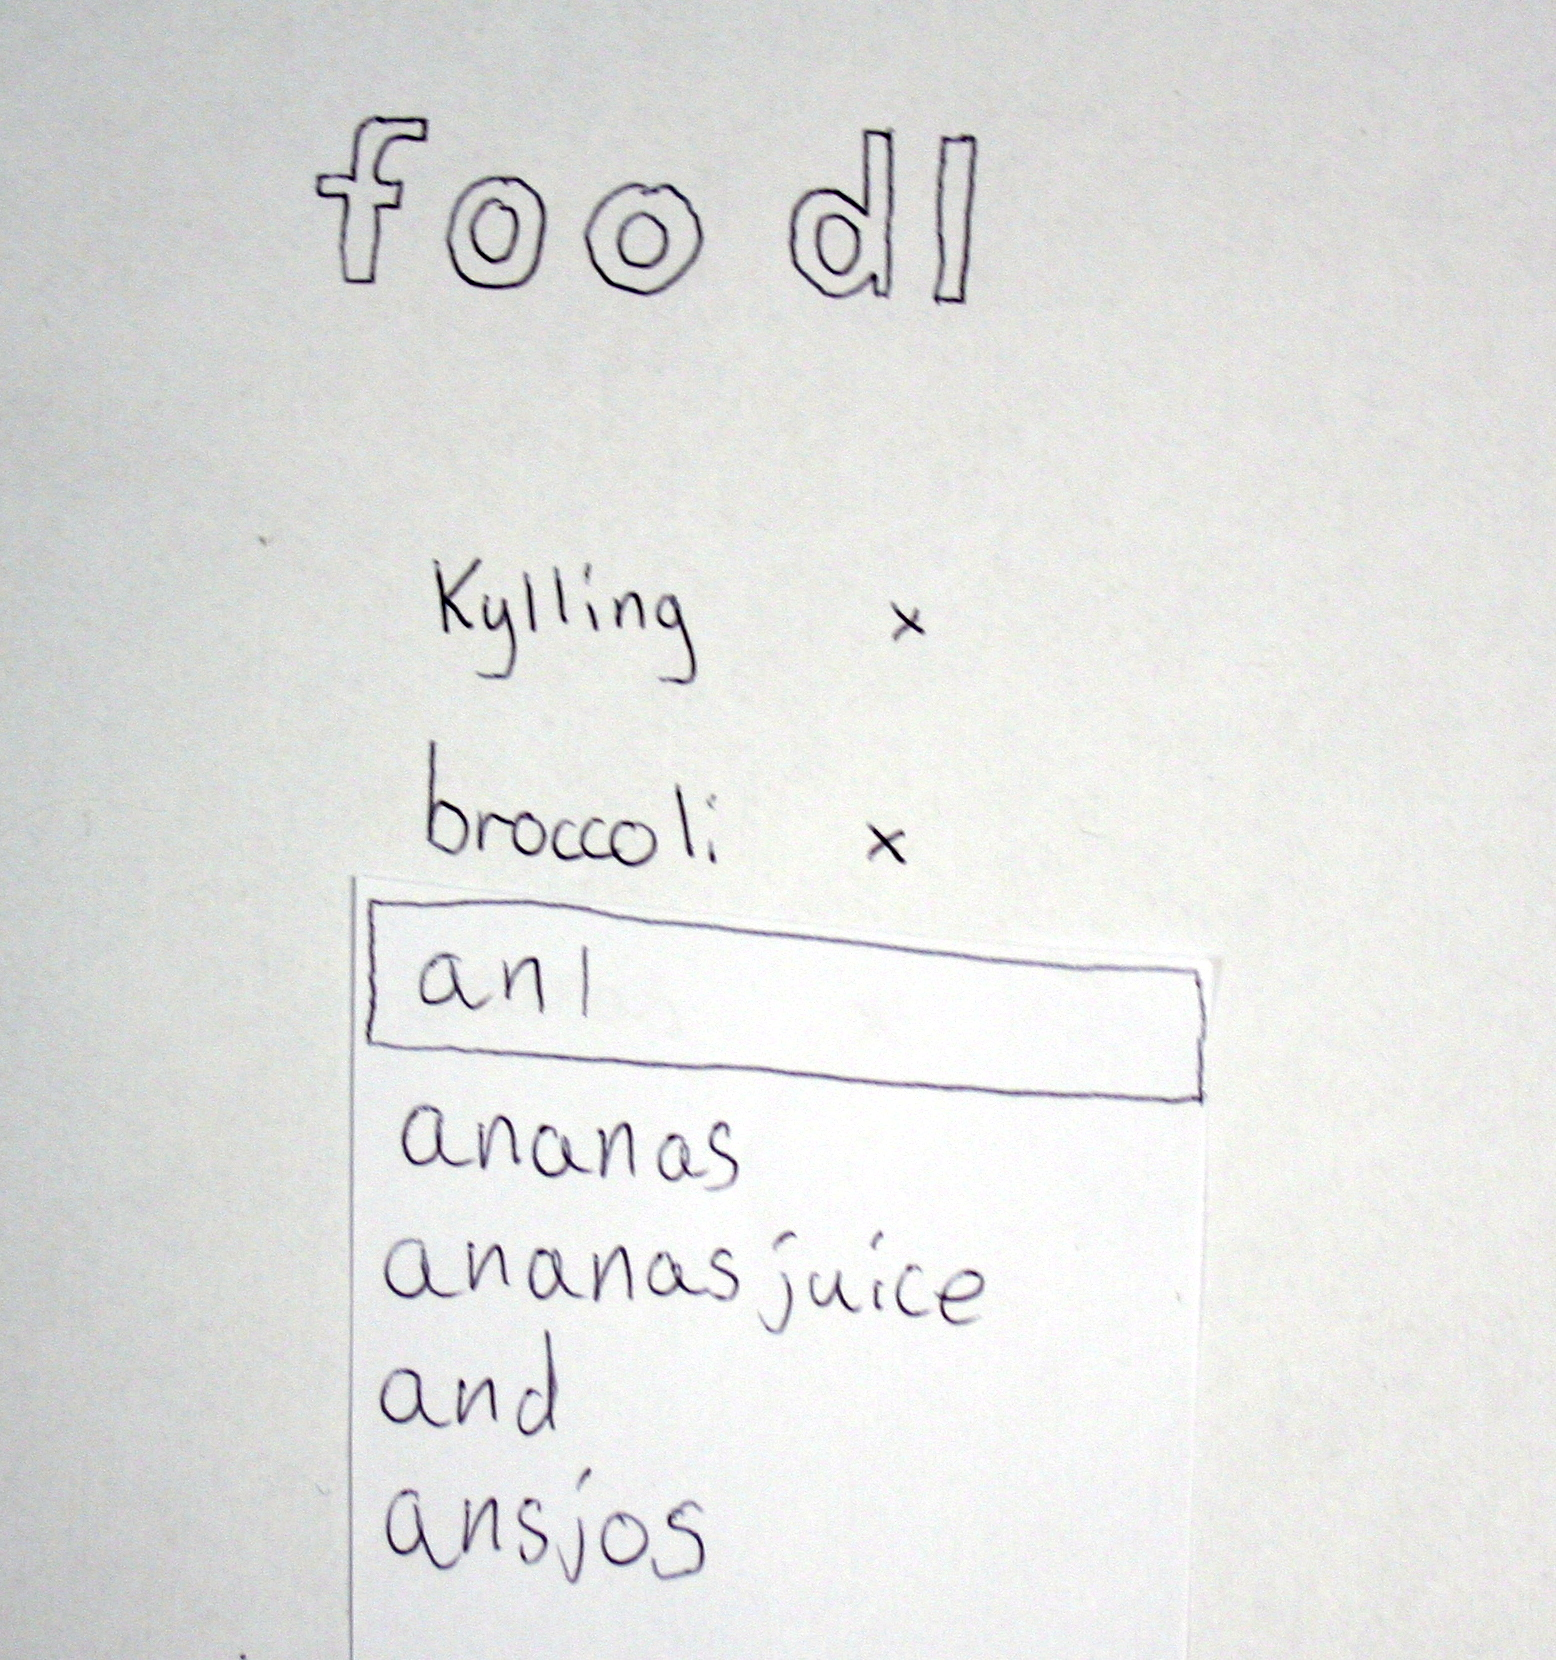
\includegraphics[width=0.5\textwidth]{billeder/prototyper/prototype1a.jpg}
\capt{Visualisering af prototype 1A.}
\label{fig:prototype1a}
\end{figure}

Præsenterer en søgeboks for brugeren, der minder meget om Google’s søgefelt. Når man indtaster et bogstav, fx “k”, kommer der en række forslag frem, såsom kylling og kartoffel, også på samme måde som ved Google, blot med den forskel at der kun foreslås ingredienser. Man kan nu klikke på forslaget eller trykke enter. Man kan også skrive ingrediensens navn færdig manuelt.

Tanken bag denne metode er at man hurtigt kan indtaste en ingrediens hvis man blot ved hvordan de første få bogstaver staves. Brugeren har med stor sandsynlighed kendskab til denne metode, da den bruges af Google, og samtidig har vi også konstrueret logoet og sidens design så det også minder om Google, netop for at gøre det intuitivt for brugeren.

Ulempen er at man har brug for et tastatur og skal tænke over hvordan man staver til ingrediensen. Det er også muligt at overse forslagene og tro man er nødsaget til at stave et meget langt ord, som for eksempel 

\item[Prototype 1B]

\begin{figure}[H]
\centering
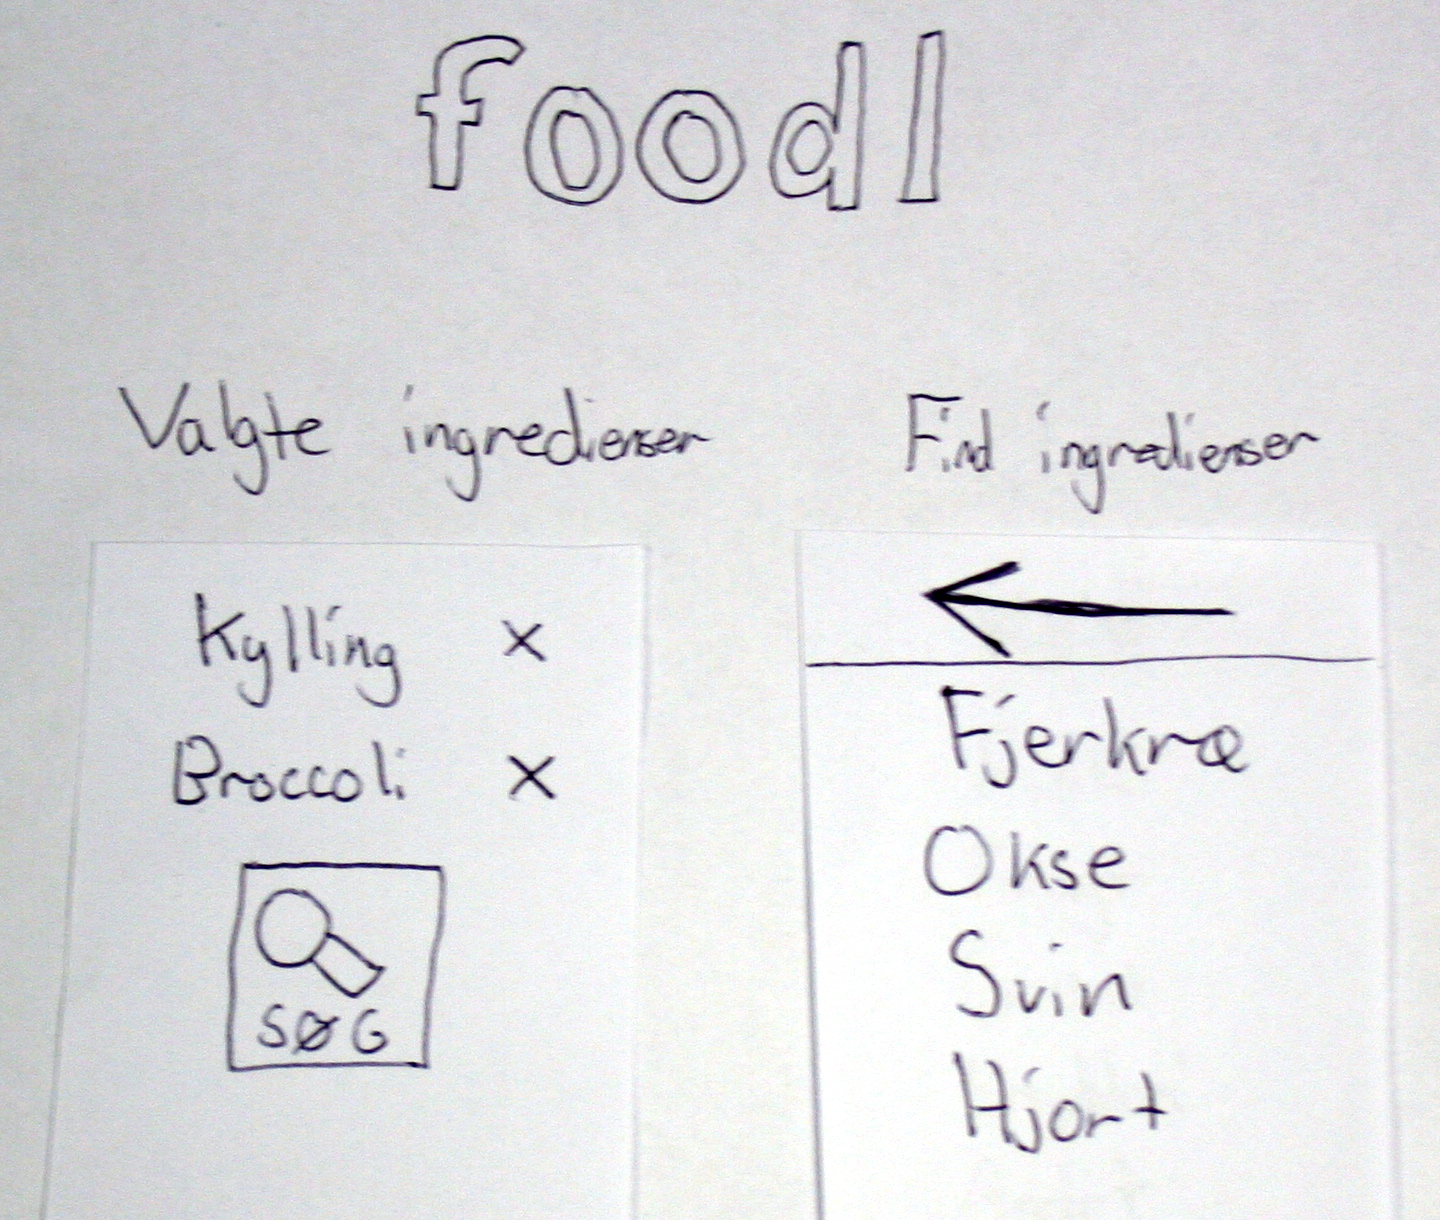
\includegraphics[width=0.5\textwidth]{billeder/prototyper/prototype1b.jpg}
\capt{Visualisering af prototype 1B.}
\label{fig:prototype1b}
\end{figure}

Fokuserer på et valg af ingredienser blandt kategorier. Man vælger først en bred kategori, som for eksempel fjerkræ, kød, brød, frugt og grønt. Dernæst vælger man et antal gange en underkategori, indtil man til sidst kan vælge en ingrediens fra en liste.

Fordelen ved denne metode er at brugeren ikke har behov for et tastatur. Det er også nemt at benytte på tablets og smartphones, da der kan skal klikkes. Ulempen er muligheden for mange kategori og forvirring omkring hvilken kategori en ingrediens findes i. Måske vil den sidste kategori der vælges stadig indeholde rigtig mange ignredienser, sådan at man skal bladre i denne liste for at finde den ønskede ingrediens. 

\item[Sammendrag] Prototype 1A var hurtig, nem og effektiv. Informanten kunne bedst lide denne metode, og hun havde ikke brug for vejledning for at kunne finde de 3 ingredienser kylling, ananas og broccoli.

Prototype 1B var langsommere at bruge og informanten syntes ikke om den. Hun var i tvivl om hvilken kategori hun skulle vælge kylling under. Kategorierne kan laves på mange forskellige måder, og uanset hvordan de vælges, vil der med garanti være nogle brugere der er i tvivl om hvor de skal lede efter en bestemt ingrediens. Et eksempel kan være kartoffelstivelse. Nogle vil lede efter kartoffelstivelse i kategorien grøntsager (fordi kartofler findes der), mens andre måske vil lede efter en kategori med navnet brød og gryn.

På baggrund af informantens valg, vælger vi at benytte metoden fra prototype 1A til at vælge ingredienser.
\end{description}

\section{Prototype 2}

Afprøvning af prototype 2 m/ fokus på systemets funktioner

\begin{description}
\item[Formål] På baggrund af møde 2, hvor informanterne kom med krav til systemets funktioner, har vi nu lavet en diasshow-prototype på gomockingbird.com, hvor systemets funktion er vist. Når informanterne præsenteres for funktionerne i noget der, med lidt god vilje, ligner et rigtigt program, så kan det være at informanten bliver klar over at en funktion enten mangler, eller at en tidligere foreslået funktion er overflødig. Formålet med mødet er derfor primært at ud af, om der er de funktioner, som informanten har brug for. Derudover vil vi også gerne finde ud af om brugeren kan finde de nødvendige funktioner, altså om programmet og dets funktioner som helhed er intuitive at bruge for informanterne.

\begin{figure}[H]
\centering
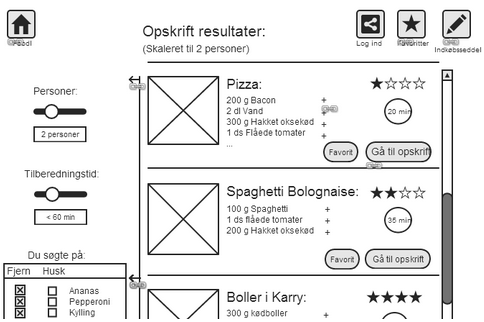
\includegraphics[scale=0.7]{billeder/prototyper/prototype2.png}
\capt{Visualisering af prototype 2.}
\label{fig:prototype2}
\end{figure}

Først udføres en case for at få ledt brugeren rundt blandt alle funktionerne.

\item[Case] Følgende case blev udført af informanterne.

\begin{enumerate}[noitemsep]
\item Udfør en søgning på ingredienserne (pepperoni, ananas og kylling). Ingredienser tilføjes ved at klikke i søgefeltet
\item Skjul alle opskrifter med nødder
\item Gå til den første opskrift, der fremkommer
\item Gå tilbage og tilføj 200 g Bacon (fra pizzaens ingredienser) til din indkøbsliste
\item Print indkøbslisten ud
\item Gør klar til en helt ny søgning
\item Foretag en søgning på pepperoni
\item Du fandt ingen opskrifter, så du vil gerne tilføj ananas, inden du søger igen (du søger altså på pepperoni og ananas)
\item Føj den første opskrift, du finder, til dine favoritter
\end{enumerate}

Efter casen tages en snak om hver af disse funktioner og muligheder med systemet.

Informanten bliver præsenteret for mange funktioner, hvor vi her beskriver hvad deres mening var omkring disse funktioner efter at have udført casen.

\begin{itemize}[noitemsep]
\item Begrænse søgeresultat efter tilberedningstid
\begin{itemize}[noitemsep]
\item Merete synes idéen er god, men foreslår nu kun 2 valgmuligheder ``kort'' eller ``lang'' tilberedningstid
\item Keld synes også dette er en god ide. En opdeling på en 30 min. burde være fint, måske 15 min. Hvis det er tilberedningstid på over en time, må skalaen godt springe mere end 15-30 min.
\end{itemize}
\item Sidebar
\begin{itemize}[noitemsep]
\item Merete opdagede ikke at denne sidebar kunne trækkes ud
\item Den ligger ikke logisk for en. Selvom den er stor. Den bliver skjult i designet
\item Keld synes ikke det ser for rodet ud, selvom sidebaren er ude hele tiden
\end{itemize}
\item Skalere en opskrift til x personer
\begin{itemize}[noitemsep]
\item Merete ser det som en nyttig funktion, hun vil skalere til mellem 2-4 personer
\item Det er en god funktion, som Keld er sikker på mange vil få brug for. Opskalering til 5 burde være nok. Måske 1-20, så er gæstebehov også dækket ind. Men det er trods alt til rester, så til 5 personer burde være nok.
\end{itemize}
\item Fjerne ingredienser inden en søgning udføres (på forsiden)
\begin{itemize}[noitemsep]
\item Merete synes det er meget brugbart
\item Keld synes det er fint at det er på forsiden
\end{itemize}
\item Fjerne ingredienser efter en søgning er udført (på søgeresultatsiden)
\begin{itemize}[noitemsep]
\item Merete synes idéen med at kunne fjerne ingredienser mens der vises søgeresultater er god
\item Keld synes det er fint, at det også er muligt i sidebaren
\end{itemize}
\item Huske ingredienser til næste søgning
\begin{itemize}[noitemsep]
\item Merete synes måden det fungerer på i prototypen er god. Hun vil ikke have at de huskede ingredienser vises på forsiden
\item Keld synes det er rart at det er muligt at huske nogle ingredienser. Det ville måske også være rart, hvis det også var muligt at gøre fra forsiden. Keld er dog i tvivl om, hvor på forsiden det skulle være. Det er måske alligevel bedst hvis forsiden er simpel. Han synes funktionen er brugbar
\end{itemize}
\item Skjule opskrifter indeholdende bestemte ting
\begin{itemize}[noitemsep]
\item Merete synes det virker godt
\item Keld synes det er en god ide. Han fik hurtigt fundet funktionen, så snart toolboxen blev åbnet
\end{itemize}
\item Browsers tilbageknap går til forsiden (beholder ingredienser)
\begin{itemize}[noitemsep]
\item Merete opdagede ikke denne funktion
\item Keld opdagede funktionen, og anvendte den også. Måske ville en tilbage- og fremknap på selve siden være brugbar, foreslår Keld
\end{itemize}
\item Home knap går tilbage (fjerne ingredienser)
\begin{itemize}[noitemsep]
\item Merete synes det virkede naturligt
\item Keld synes det er godt at have en kanp som går helt tilbage. Men han foreslår endnu engang at have en frem- og tilbageknap som supplerer home-knappen
\end{itemize}
\item Visning af opskrifter (ekspander ved mouse over)
\begin{itemize}[noitemsep]
\item Merete synes opskrifterne blev vist fint. Hun kunne godt lide idéen med at ekspandere opskriften ved mouseover
\item Keld synes bare man skal have vist de væsentligste ingredienser. Han synes det ville være smart, hvis det var muligt at se hele ingredienslisten ved hjælp af et mouse-over
\end{itemize}
\item Gå til opskrifter (evt link ved klik på navn)
\begin{itemize}[noitemsep]
\item Merete synes ikke knappen “Gå til opskrift”, er overflødig. Hun ville blive forvirret hvis den ikke var der, og man bare skulle trykke et sted på opskriften (navnet, eller baggrunden, hvor baggrundsfarve ændrer sig eller lignende)
\item Keld synes det er godt med en “Gå til opskrift”-knap. Det er brugervenligt
\end{itemize}
\item Tilføj opskrift til favoritter
\begin{itemize}[noitemsep]
\item Merete synes ikke man skal gå fra et søgeresultat og over til favoritsiden hver gang man tilføjer en opskrift til favoritter. Opskriften skal blot tilføjes. Måske den skal sige en lyd og fjerne knappen man trykkede på. Favoritter-ikonet kunne lyse op
\item Skal lave en “Fjern fra favorit-knap”, så man hurtigt kan ombestemme sig
\item Keld synes det er smart nok at man sendes ind på favoritlisten, så man er sikker på at opskriften er kommet derind. Havde man samtidig en frem- og tilbageknap ville det være endnu bedre
\end{itemize}
\item Favoritter (knappen, der viser ens favoritter)
\begin{itemize}[noitemsep]
\item Merete var lidt forvirret med hensyn til om den tilføjede en opskrift til favoritter, eller hvad den gjorde
\item Keld synes at det skal være muligt at skalere opskrifterne på favoritsiden og at det er muligt nemt at fjerne opskrift fra favoritsiden igen
\end{itemize}
\item Visning af favoritter (layout)
\begin{itemize}[noitemsep]
\item Merete syntes layoutet var godt, og kunne godt lide at det mindede om layoutet ved visning af søgeresultat
\item Keld synes godt om layoutet
\end{itemize}
\item Visning af indkøbsliste
\begin{itemize}[noitemsep]
\item Merete synes det er en god idé at man kan tilføje tekst
\item Keld foreslår at man har ingredienslisten fra den opskrift man har været inde på, ved siden af indkøbslisten, så det er muligt hurtigt at tilføje flere ingredienser derfra
\item Keld synes indkøbslisten er meget brugbar. Det er for ofte man glemmer nogle ting, uden indkøbslisten
\end{itemize}
\item Tilføje opskrifts ingredienser til indkøbsliste
\begin{itemize}[noitemsep]
\item Merete vidste ikke hvordan man gjorde. Hun troede ikke man kunne trykke på +’et
\item Keld kunne godt tilføje en ingrediens til indkøbslisten
\end{itemize}
\item Home-knappen sender en til en helt tom forside
\begin{itemize}[noitemsep]
\item Merete kunne godt lide dette. Det virkede helt naturligt for hende
\item Keld synes det giver mening
\end{itemize}
\item Logge ind (få afklaret med brugeren, hvordan det skal foregå)
\begin{itemize}[noitemsep]
\item Log ind mest forståeligt
\item Kender meget til login, intet til synkronisering
\item Log ind er klart mest forståeligt for Keld. Keld har ikke lyst til at indtaste mere end mail-adresse, navn eller brugernavn og adgangskode. Helst ikke mere end det. Det er fint at der kommer en bekræftelsesmail til ens indbakke, men helst ikke aktiveringsmail
\item Sikkerheden har ikke høj-prioritet for Keld, da der alligevel ikke er nogle følsomme informationer på siden
\end{itemize}
\item Informants forslag til flere funktion
\begin{itemize}[noitemsep]
\item Merete havde ingen forslag, udover at der skal være billede af opskrifterne, hvilket ikke var vist i prototypen
\item Keld foreslår at sidebaren også er på favoritsiden
\item Keld foreslår en frem- og tilbageknap
\item Filtrering af forskellige landes køkkener, så det eksempelvis var muligt at se italienske retter, kinesiske retter osv. (kun de mest kendte køkkener: nordiskekøkken, kinesiske, italienske, græske \fx)
\end{itemize}
\end{itemize}
\end{description}

\subsection{Sammendrag}

I forhold til funktionalitet i prototypen, er der nogle få ting, der skal tilføjes, fjernes eller ændres

\begin{enumerate}[noitemsep]
\item Når man på søgesiden tilføjer en opskrift til favoritter, skal man forblive på søgesiden. Knappen man trykkede på skal erstattes med en ``Fjern fra favoritter''-knap
\item Sidebaren på søgeresultatssiden skal være nemmere at få øje på. En løsning er at gøre den synlig fra starten og give brugeren muligheden for at skjule den
\item Knappen i toppen, der viser de favoritter man har gemt, skal være mere sigende. ``Vis favoritter'' kunne der stå under den
\item På søgeresultatsiden, hvor en opskrifts vises, skal +’et ud for ingredienserne, der tilføjer en ingrediensen til indkøbslisten, være mere intuitiv
\item Brugeren skal muligvis have at vide, at man kan benytte browserens tilbageknap for at gå tilbage til forsiden, uden at ingredienser fjernes. Det kan være at informanten overså denne funktion fordi prototypen blev vist i form af et diasshow på en hjemmeside, og informanten derfor var bange for at gå væk fra hele diasshowets side
\item Skalering og andre funktioner til visning af favoritter
\item Frem og tilbage knap, der giver brugeren tryghed når han navigerer rundt, så man ikke skal være bange for at browseren forsvinder fra siden
\end{enumerate}

%\section{Supplerende spørgsmål}

Her findes spørgsmål, der løbende er blevet stillet informanterne, ved tvivlstilfælde udenfor planlagte møder.

Formål: At afklare om klassen indkøbsliste i problemområdet skal aggregere en råvaretype-, en ingrediensklasse eller begge dele.
Os: ``Lad os sige, at du har fundet en opskrift du gerne vil købe ind til. Du beslutter dig for at lave en indkøbsliste, så du kan huske hvad du skal købe for at lave opskriften. Vil du skrive på indkøbslisten, hvor meget du skal købe af de forskellige ingredienser?''
Merete: ``Ja, det vil jeg helt klart, ellers ville jeg være bange for at glemme hvor meget jeg har brug for.''


\chapter{Manuel mapping}
\label{ap:manuel-mapping}

\begin{figure}
\centering
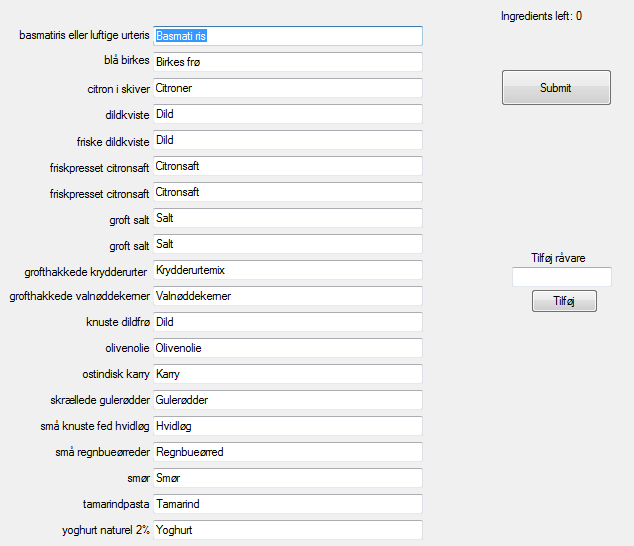
\includegraphics[scale=0.6]{billeder/manuel-mapping.png}
\capt{Program skrevet i C\# til kontrol og remapping af ingredienser}
\end{figure}


\chapter{Valg af mapping metode}
\label{ap:valgafmappingmetode}

\begin{figure}
\centering
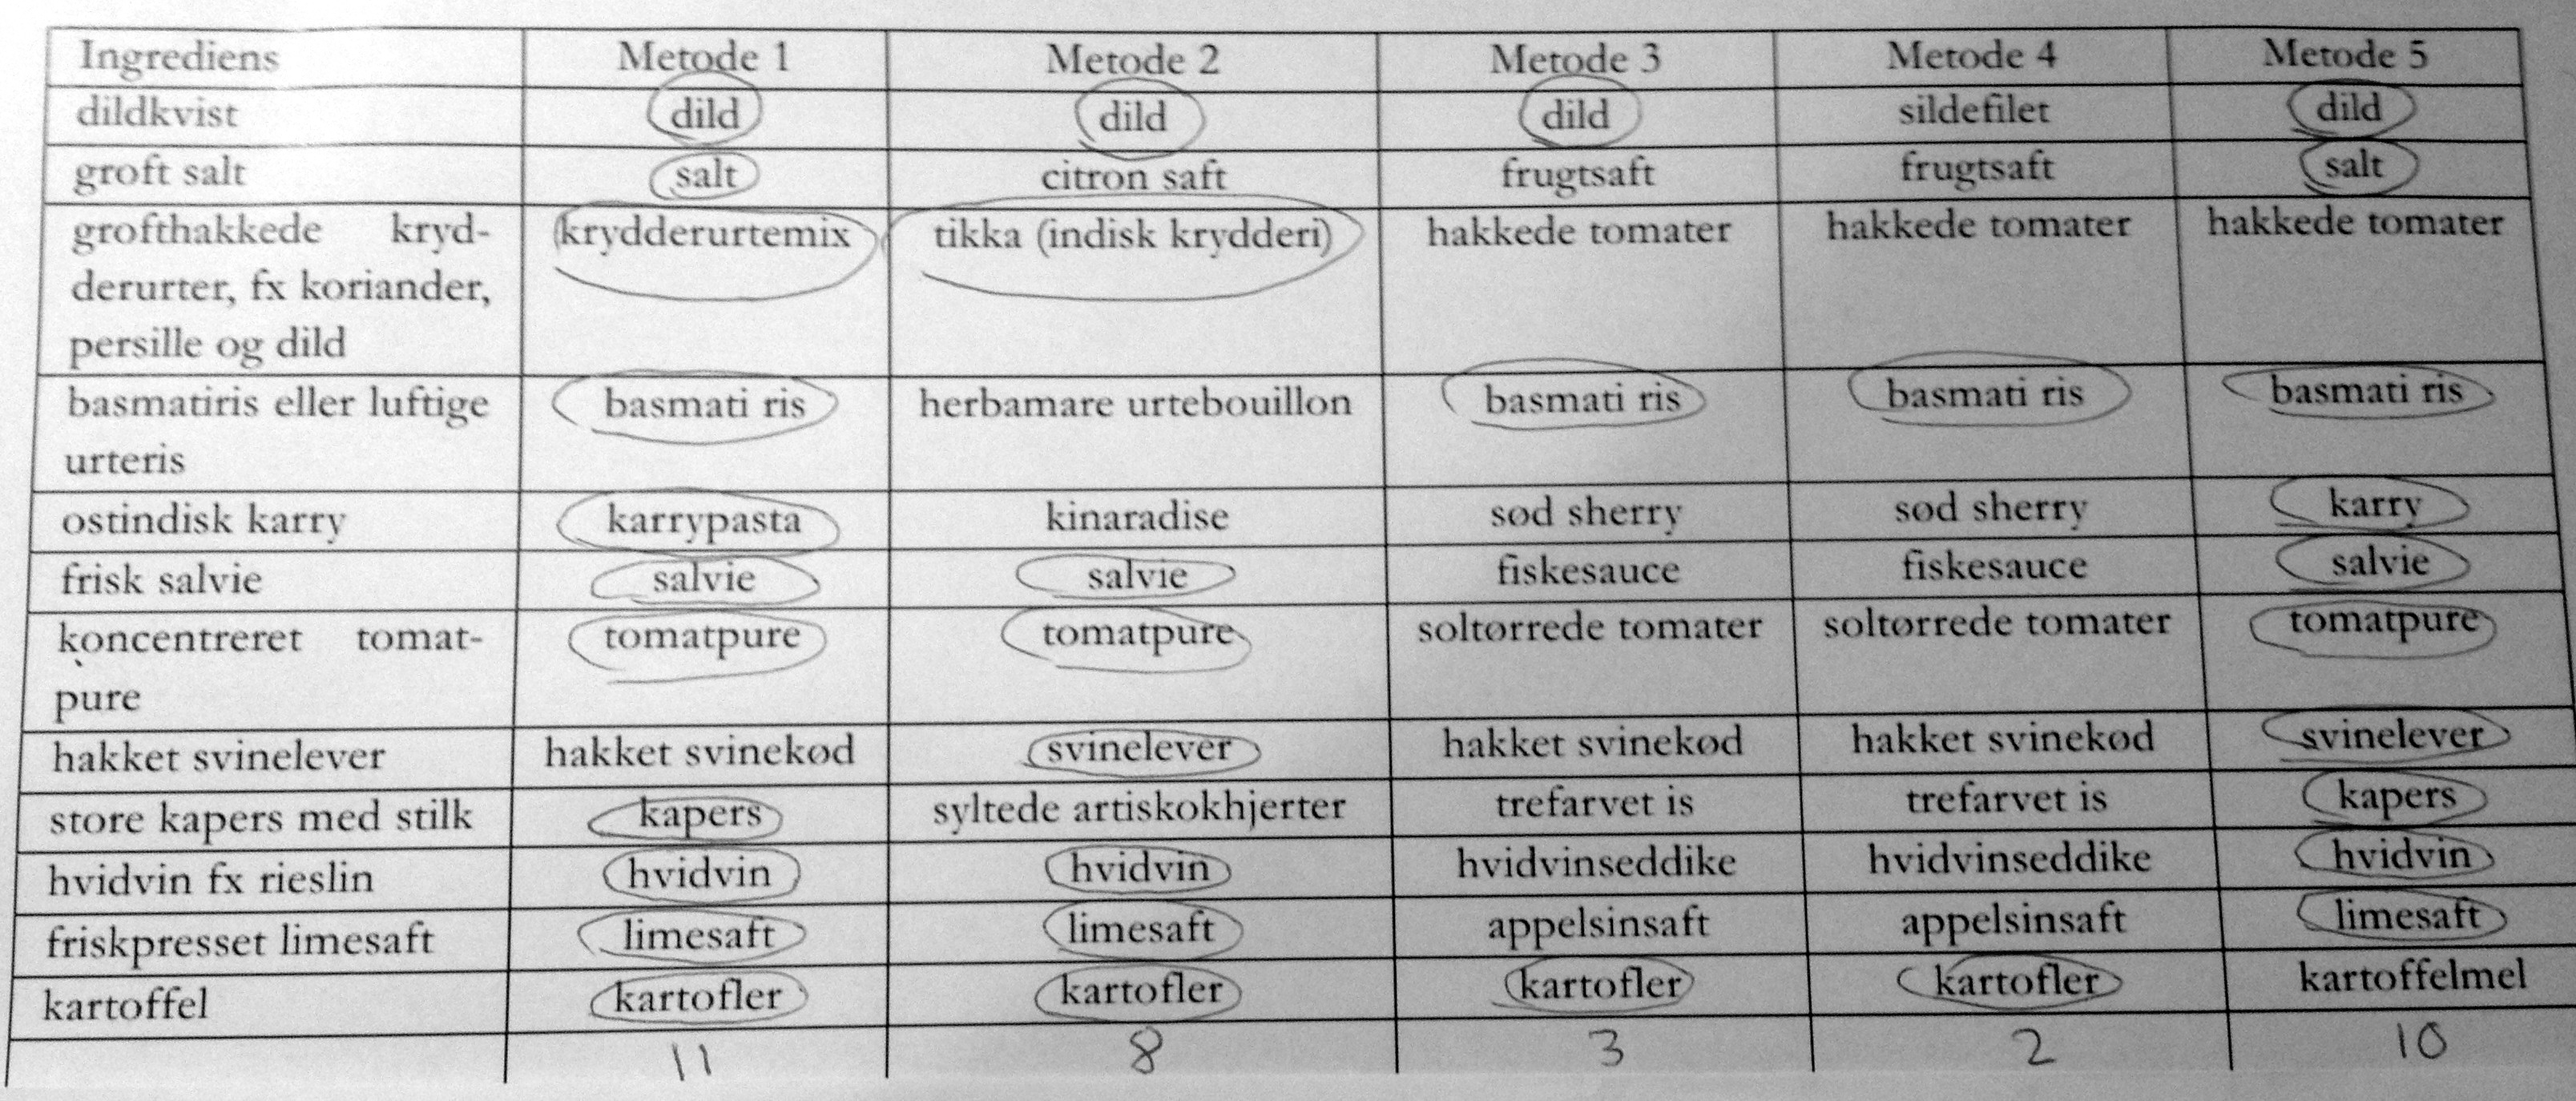
\includegraphics[width=0.8\textwidth]{billeder/valgafmappingmetode.jpg}
\capt{Informanterne satte ring om de mappings, de mente var korrekte. }
\end{figure}


\end{document}
